\documentclass[12pt]{article}
\usepackage[]{color}
%\usepackage[document]{ragged2e} % for left-aligning, helpful when opening in Word later


%% maxwidth is the original width if it is less than linewidth
%% otherwise use linewidth (to make sure the graphics do not exceed the margin)
\makeatletter
\def\maxwidth{ %
	\ifdim\Gin@nat@width>\linewidth
	\linewidth
	\else
	\Gin@nat@width
	\fi
}
\makeatother

\definecolor{fgcolor}{rgb}{0.345, 0.345, 0.345}
\newcommand{\hlnum}[1]{\textcolo!r[rgb]{0.686,0.059,0.569}{#1}}%
\newcommand{\hlstr}[1]{\textcolor[rgb]{0.192,0.494,0.8}{#1}}%
\newcommand{\hlcom}[1]{\textcolor[rgb]{0.678,0.584,0.686}{\textit{#1}}}%
\newcommand{\hlopt}[1]{\textcolor[rgb]{0,0,0}{#1}}%
\newcommand{\hlstd}[1]{\textcolor[rgb]{0.345,0.345,0.345}{#1}}%
\newcommand{\hlkwa}[1]{\textcolor[rgb]{0.161,0.373,0.58}{\textbf{#1}}}%
\newcommand{\hlkwb}[1]{\textcolor[rgb]{0.69,0.353,0.396}{#1}}%
\newcommand{\hlkwc}[1]{\textcolor[rgb]{0.333,0.667,0.333}{#1}}%
\newcommand{\hlkwd}[1]{\textcolor[rgb]{0.7te37,0.353,0.396}{\textbf{#1}}}%

%\usepackage{framed}
%\makeatletter
%\newenvironment{kframe}{%
%	\def\at@end@of@kframe{}%
%	\ifinner\ifhmode%
%	\def\at@end@of@kframe{\end{minipage}}%
%\begin{minipage}{\columnwidth}%
%	\fi\fi%
%	\def\FrameCommand##1{\hskip\@totalleftmargin \hskip-\fboxsep
%		\colorbox{shadecolor}{##1}\hskip-\fboxsep
%		% There is no \\@totalrightmargin, so:
%		\hskip-\linewidth \hskip-\@totalleftmargin \hskip\columnwidth}%
%	\MakeFramed {\advance\hsize-\width
%		\@totalleftmargin\z@ \linewidth\hsize
%		\@setminipage}}%
%{\par\unskip\endMakeFramed%
%	\at@end@of@kframe}
%\makeatother

\definecolor{shadecolor}{rgb}{.97, .97, .97}
\definecolor{messagecolor}{rgb}{0, 0, 0}
\definecolor{warningcolor}{rgb}{1, 0, 1}
\definecolor{errorcolor}{rgb}{1, 0, 0}
\newenvironment{knitrout}{}{} % an empty environment to be redefined in TeX

%%% FONT AND INPUT
\usepackage[T5]{fontenc}
\usepackage[utf8]{inputenc} % set input encoding (not needed with XeLaTeX)

%%% Examples of Article customizations
% These packages are optional, depending whether you want the features they provide.
% See the LaTeX Companion or other references for full information.

%%% PAGE DIMENSIONS
\usepackage{geometry} % to change the page dimensions
\geometry{letterpaper} % or letterpaper (US) or a5paper or....
\geometry{margin=1in} % for example, change the margins to 2 inches all round
% \geometry{landscape} % set up the page for landscape
%   read geometry.pdf for detailed page layout information

\usepackage{graphicx} % support the \includegraphics command and options

% \usepackage[parfill]{parskip} % Activate to begin paragraphs with an empty line rather than an indent

%%% PACKAGES
\usepackage{booktabs} % for much better looking tables
\usepackage{array} % for better arrays (eg matrices) in maths
\usepackage{paralist} % very flexible & customisable lists (eg. enumerate/itemize, etc.)
\usepackage{verbatim} % adds environment for commenting out blocks of text & for better verbatim
\usepackage{subcaption} % make it possible to include more than one captioned figure/table in a single float
\usepackage{float}
\usepackage{setspace}
\usepackage{amsmath,newtxtext,newtxmath}
\usepackage{url}
\usepackage{multirow}
\usepackage{listings}
\usepackage{dcolumn}
%\usepackage[nolists]{endfloat}
\usepackage{bbm}
\usepackage{pdflscape}
\usepackage{pdfpages}
\usepackage{afterpage} % to flow paragraph through full-page landscape table
\usepackage{xr} % to use \ref with labels from the main text
\externaldocument{'210102 - JOP RnR Draft 1 Appendix'}
\usepackage{tikz} 
\usetikzlibrary{arrows,decorations.pathmorphing,decorations.pathreplacing,backgrounds,fit,positioning,shapes.symbols,chains}


%%% WATERMARK

%\usepackage{draftwatermark}
%\SetWatermarkText{DRAFT - FOR HANNAH M.}
%\SetWatermarkScale{.25}

%%% HEADERS & FOOTERS
\usepackage{fancyhdr} % This should be set AFTER setting up the page geometry
\pagestyle{fancy} % options: empty , plain , fancy
\renewcommand{\headrulewidth}{0pt} % customise the layout...
\lhead{}\chead{}\rhead{}
\lfoot{}\cfoot{\thepage}\rfoot{}

%%% CITATION AND BIBLIOGRAPHY

\usepackage[authordate,backend=bibtex8,natbib,sorting=nyt,sortcites,isbn=false,doi=false,citecounter=true,noibid,date=year]{biblatex-chicago}
%\usepackage{natbib}
%\bibliographystyle{apsr}
\bibliography{Literature/library_syp}

%\renewcommand{\finentrypunct}{%
%	\addperiod\space
%	(Cited \arabic{citecounter}~time\ifnumequal{\value{citecounter}}{1}{}{s})%
%}

% fix problem with \citeyear and \citeyearpar not being highlighted
\DeclareCiteCommand{\citeyear}
	{}
	{\bibhyperref{\printdate}}
	{\multicitedelim}
	{}

\DeclareCiteCommand{\citeyearpar}
	{}
	{\mkbibparens{\bibhyperref{\printdate}}}
	{\multicitedelim}
	{}
% possessive cite with \citepos
\newcommand\citepos[1]{\citeauthor{#1}'s\ (\citeyear{#1})}

% change fnote style to normal text, double-spaced
\renewcommand{\footnotesize}{\normalsize}
\newcommand\fnote[1]{\footnote{\baselineskip=2\normalbaselineskip#1}}
\setlength{\footnotesep}{2pc}

\usepackage{hyperref}
\hypersetup{
	colorlinks=true,
	linkcolor=blue,
	filecolor=magenta,      
	urlcolor=cyan,
}

%%% SECTION TITLE APPEARANCE
\usepackage{sectsty}
%\allsectionsfont{\sffamily\mdseries\upshape} % (See the fntguide.pdf for font help)
\sectionfont{\fontsize{14}{15}\rmfamily\bfseries\upshape}
\subsectionfont{\fontsize{13}{15}\rmfamily\mdseries\slshape}

% (This matches ConTeXt defaults)

%%% ToC (table of contents) APPEARANCE
\usepackage[nottoc,notlof,notlot]{tocbibind} % Put the bibliography in the ToC
\usepackage[titles,subfigure]{tocloft} % Alter the style of the Table of Contents
\renewcommand{\cftsecfont}{\rmfamily\mdseries\upshape}
\renewcommand{\cftsecpagefont}{\rmfamily\mdseries\upshape} % No bold!

%%% Some commands
\newcommand{\reg}{\texttt{regress} }
\newcommand{\1}{\mathbbm{1}}

\renewcommand\r{\right}
\renewcommand\l{\left}
\newcommand\E{\mathbbm{E}}
\newcommand\V{\mathbbm{V}}
\newcommand\Var{\mathbbm{V}}
\newcommand\avar{{\rm Avar}}
\newcommand\dist{\buildrel\rm d\over\sim}
\newcommand\iid{\stackrel{\rm i.i.d.}{\sim}}
\newcommand\ind{\stackrel{\rm indep.}{\sim}}
\newcommand\cov{{\rm Cov}}
\newcommand{\R}{\textbf{R} }
\newcommand{\Rcmd}[1]{{\large \texttt{#1}}}
\newcommand\indep{\protect\mathpalette{\protect\independenT}{\perp}}
\def\independenT#1#2{\mathrel{\rlap{$#1#2$}\mkern2mu{#1#2}}}
\DeclareMathOperator{\sgn}{sgn}
\DeclareMathOperator*{\argmin}{argmin}

\newcommand\Sum{\sum^N_{i=1}}
\newcommand\Prod{\prod^N_{i=1}}
\newcommand{\pderiv}[1]{\frac{\partial}{\partial #1}}
\newcommand{\B}[1]{\boldsymbol{#1}}
\newcommand{\logit}{\text{logit}}

% Set this to 1 to use end notes and place tables and figures at the end
\newcommand{\manuscript}{0}

\if\manuscript1
\usepackage[nolists,tablesfirst]{endfloat} % to place tables and figures at the end
\usepackage{endnotes} % to convert footnotes to endnotes
\let\footnote=\endnote
\fi

%%% texcount
% Run texcount on tex-file and write results to a sum-file
\immediate\write18{texcount  \jobname.tex -out=\jobname.sum -incbib -relaxed}
% Define macro \wordcount for including the counts
\newcommand\wordcount{\verbatiminput{\jobname.sum}}

%%%%opening

\title{Tea Leaf Elections: \\
	Inferring Purpose for Authoritarian Elections from Post-election Responses to Defeats%
%	\thanks{I am grateful to Christina Alvarez-Mongote, Julie Bunck, Daniel Hidalgo, Andrew Halterman, Sean Liu, Edmund Malesky, Blair Read, Paul Schuler, Lily Tsai, and participants at MIT Second-Year Paper Workshop and the MPSA Conference 2019, and three anonymous reviewers for their guidance and feedback. Ngoc Phan and Edmund Malesky provided me with the data on Vietnamese government officials.}
	\\
	\vspace{2ex}
	\vphantom{Online Appendix}}
%\author{Minh D. Trinh%
%	\thanks{Doctoral Candidate, Department of Political Science, Massachusetts Institute of Technology. 30 Wadsworth Street E53-415, Cambridge, MA 02142. Phone number: +1-857-600-9241. E-mail: \url{mdtrinh@mit.edu}.}}
\date{January 15, 2020}

\begin{document}
	
%TC:ignore 

\maketitle
\thispagestyle{empty}
\doublespacing

% uncomment this to print title page only
%\end{document}

% change font typeface and size for proofreading
%\sffamily
%\large

\begin{abstract}
The power of authoritarian elections is not unlimited. When using elections as a source of information, authoritarian regimes may not be able to collect from a single election all the information it could theoretically provide, and so they must commit to seeking only some specific signal(s) in each election. It is possible to identify the type of information each regime seeks from its elections by studying its reactions to small but unexpected defeats. Applying this logic to Vietnam, I find that the regime responded to the defeats of its favored candidates in the 2016 election for the national legislature by increasing central transfers to provinces where it suffered these defeats. This evidence suggests that the Vietnamese regime uses elections as an opinion poll to identify areas in which it is less popular, instead of as a test to detect local officials who under-perform in their electoral mobilization efforts.
\end{abstract}

%Word count: 10,490

%TC:endignore 

\newpage

\pagenumbering{arabic}

%\section*{Introduction}

At first glance, authoritarian elections seem to be a powerful weapon in the dictator's arsenal: not only do they rarely pose existential threats, but these elections also cement autocrats' rule by providing critical information otherwise unknowable about influential forces both internal and external. The literature that explores authoritarian elections' many informational functions, however, has not considered potential conflicts between such functions. Autocrats cannot expect authoritarian elections to be informative by default, but must engineer their elections in specific ways to make them informative. However, an election that is engineered to provide information on some aspects of governance may become less effective at shedding light on others. This forces authoritarian rulers to set priorities and use elections as a telescope focused on a few areas of interest, rather than a panoramic camera that captures every detail that comes into view.

Without directly observing autocrats' thought processes, how can outside observers know which type of information is being collected through an authoritarian election? In this paper, I propose a framework through which to identify potentially informative elections and find which specific informational goal(s) they serve. Applying this framework to the case of Vietnam, I show that the Communist Party of Vietnam (CPV) needs information on both the sub-national distribution of regime support and the quality of its provincial officials but only uses elections to learn about the former. I take advantage of the rare and unexpected defeats of regime-favored candidates in Vietnam's 2016 legislative election, and show that the CPV increased central transfers to provinces with such defeats. This finding corroborates the hypothesis that the regime saw election defeats as indicators for pockets of disillusioned citizens and spent money to placate them but rejects the hypothesis that it used these defeats to identify and punish under-performing provincial executives. %Under this alternative hypothesis the CPV would have wanted to punish officials in these provinces, but the increased central transfers would have accomplished only the opposite.

This paper contributes to the larger literature on authoritarian institutions by demonstrating how existing theories about authoritarian elections' functions may contradict each other in some specific contexts--specifically those that portray elections as the autocrat's opinion poll \citep[e.g.][]{Miller2015, Magaloni2006, Blaydes2010} and those that portray them as a test to evaluate regime agents \citep[e.g.][]{Magaloni2006, Blaydes2010,Myagkov2009,RundlettSvolik2016}. In addition, it offers a framework through which to identify autocrats' motivations and test theories of authoritarian elections using post-election responses to localized defeats. Finally, the findings illustrate that even stable authoritarian regimes like Vietnam may still respond to public dissatisfaction, suggesting pathways for accountability via formal authoritarian institutions.

%\section*{The Information Limits of Authoritarian Elections Informative}
%\label{sec:lit_review}

\section*{The Informational Limits of Authoritarian Elections}
\label{sec:theory_limits}

Why do some authoritarian regimes choose to hold elections, and then allow less-than-satisfactory results to happen, when they could have gotten away without them? The literature on authoritarian elections has proposed that elections may confer enough benefits for autocrats to justify their potential risks.\fnote{See \citet{LustOkar2005, AR2005, Magaloni2006, Blaydes2010, Miller2015, Cox2009, Geddes2018} for some seminal works.} Notably, this literature shows that authoritarian elections provide autocrats with different types of information, such as about their opponents' strength \citep[][Ch. 6]{Geddes2018}, the existence of potential threats or allies \citep{LustOkar2005}, the competence or loyalty of their agents \citep{Magaloni2006, Blaydes2010, Myagkov2009, RundlettSvolik2016}, the citizenry's \textit{level} of dissatisfaction with the regime \citep{Miller2015} or even its \textit{distribution} across sub-national units \citep{Magaloni2006, Blaydes2010}. All this information then contributes to authoritarian longevity by allowing the regime to adjust its policies, by suppressing opposition strongholds \citep{Magaloni2006, Blaydes2010}, buying off a dissatisfied public \citep{Miller2015, Magaloni2006}, or co-opting emerging elites into the regime \citep{LustOkar2005}.

Other scholars \citep[e.g.][]{Rozenas2016, Wintrobe2000, Morgenbesser2016}, however, argue that good information does not emerge easily from authoritarian elections. They note an important trade-off between authoritarian elections' primary functions: an election can only be informative about an internal or external force if this force is allowed to manifest in the vote count; for this to happen election results must vary as an unknown function of that force.\footnote{\citet{Little2017} models the informativeness of an election as the variance of its expected result.} Thus, autocrats who manipulate elections to win them only end up lowering these elections' information value. In the most extreme case, incumbents who always know they would win 100\% of the votes--such as in North Korea--receive no new information about the country's internal politics from this outcome.

In light of these opposing viewpoints, I posit these elections may provide information to autocrats but such informational value is severely limited. Specifically, I argue that among the many different types of information that authoritarian elections may bring, autocrats can only seek a few and must forfeit the rest. Instead, an election that seeks to be a jack of all trades only risks becoming a master of none: the more kinds of information a dictator seeks from an election, the less effective it becomes at providing any of them. There are several reasons for this phenomenon:

First, information from elections--in particular information from election results--is inherently complex. At their core, election results consist of sets of raw numbers that require interpretation. When there are multiple potential ways to interpret a particular set of results, solid conclusions are no longer possible. \citet[][461]{Gandhi2015} notes this over-determination problem by highlighting how the opposition's success in the 2002 Kenyan elections could be due to \textit{``external pressure, the defection of regime insiders, the coordination of opposition efforts, or any combination of these factors.''} Similarly, when an authoritarian regime faces a low incumbent vote count in a certain district, it may attribute this setback to regime agents failing to manipulate the election enough or particular pockets of citizens feeling disenchanted enough to risk voting against the ruling party. Depending on how the regime interprets the defeat, it may learn something about either the quality of its agents or the distribution of its popularity across the country; if both interpretations are equally plausible, the regime may have to decide which one they believe more. For example, when faced with this problem the Russian regime prioritized the first interpretation \citep[][136]{Myagkov2009}, but doing so indicated that the regime had made important but potentially unwarranted assumptions about the uniformity of its strength across the entire country.

To extract useful and unambiguous information from elections, autocrats who consciously seek information from elections typically engage in \textit{selective manipulation}, combining careful restraint in some parts of the electoral process with bold manipulation in others. Restraint is necessary because an election's results is only informative of a variable if the variable is allowed to influence the vote tally. At the same time, to ensure that election results are truly informative of any particular variable, autocrats also need manipulation tactics that prevent others from entering the equation. In this sense, strategies that place rigid controls on some moving parts of the electoral process not only help autocrats win elections, but also reduce the informational complexity of these elections. This selective manipulation logic offers another explanation for why many authoritarian regimes use only a subset of manipulation tactics available to them, such as Singapore's government tilting electoral rules to favor the ruling party but refraining from vote fraud \citep{Tan2013}, or take actions that may limit their manipulation capacity, such as welcoming international observers \citep{Little2015}.

Herein lies the second obstacle to information collection from elections: selective manipulation works best if it completely shuts down most determinants of election outcomes, yet when it does nothing can be learned about these determinants. In other words, tactics that ensure elections send clear signals about a few specific types of information but also prevent them from emitting any signal about all the others. For autocrats, deciding which manipulation tactic(s) to employ thus amounts to deciding which kind of information they can and cannot seek.

Third, selective manipulation also means selective restraint. Allowing more types of information to arise from elections means giving up more control of the electoral process, which is only feasible for a few authoritarian regimes, as they must be secure enough to tolerate some electoral risks without facing existential threats. Additionally, the regime's leaders must exercise a high degree of control over its agents through a disciplined machine, overseeing which manipulation strategies are and are \textit{not} being carried out. It is thus no surprise that existing literature has mostly documented information collection through authoritarian elections in relatively secure hegemonic, dominant-party or single-party regimes where elections are rarely competitive.
%such as Mexico \citep{Magaloni2006}, Egypt \citep{Blaydes2010}, Jordan \citep{LustOkar2005}, Russia \citep{Myagkov2009, RundlettSvolik2016}, Malaysia \citep{Brownlee2007}, Vietnam \citep{MaleskySchuler2011}, or Singapore \citep{Miller2015}. 

Furthermore, even if an authoritarian regime does not worry about losing, it may still have other goals when holding elections, some of which may be jeopardized even by a minimal extent of restraint. For instance, even as some authoritarian regimes seek legitimation by tolerating or even inviting some apparent electoral setbacks \parencite{Morgenbesser2016}, others build their legitimacy on the foundation of large or absolute victories \parencite{Simpser2013}, which reduces their ability to tolerate selective restraint and limits the range of information they could glean from elections.

Finally, there is a practical constraint: a regime seeking to infer too many different types of information from the same election may struggle to make policy adjustments to respond to all the incoming information. Specifically, when an election brings to a regime multiple different pieces of information, the logical response to one piece may end up contradicting the response to another. For example, \citet{Blaydes2010} finds that the Mubarak regime in Egypt interpreted election setbacks as evidence of opposition strongholds and disloyal ruling party members, and reacted by cutting funding and thus public services to areas in which it had suffered defeat. However, these defeats could have been a result of general citizen dissatisfaction, in which case the funding cuts would be the opposite of an appropriate response \citep{Miller2015}. The potential clash between different responses to incoming information is especially high for regimes whose capacity for action is limited, but also high-capacity regimes with highly structured institutions and minimal policy discretion. For these regimes, seeking too much information from elections only results in contradictory policy recommendations, which debilitates more than it facilitates policy responsiveness.

In sum, the limits to authoritarian elections' informational value pertain not to how many different signals an election may emit simultaneously, but rather to how many of these signals a regime can digest. Seeking too many different pieces of information from authoritarian elections muddles the quality of each piece, all while interfering with other goals for the elections and preventing effective responses to all the received information. Therefore, autocrats may find it in their best interest to limit the range of information they seek by carefully designing their selective manipulation strategies. If this is cannot be perfectly achieved, they must choose to ignore plausible interpretations of election results, and pay attention to only what they need to know, accepting the possibility of picking up the wrong information entirely.

% The solution, then, is to design their manipulation strategies to limit the range of possible information to only what they can coherently react to. If this is not possible, autocrats must willfully ignore some plausible information and pay attention to only what they need to know, accepting the possibility of learning the wrong lesson entirely. 

% In practice, other constraints or even mistakes may lead autocrats to misjudge the fine balance between manipulation and restraint. Furthermore, because autocrats may avoid some manipulation tactics for other strategic reasons, evidence of selective manipulation strongly suggests but still does not confirm that they have an informational interest in authoritarian elections.

\subsection*{Vietnam: A Single-Party Regime with Unmet Informational Needs}
\label{sec:vietnam_elections}
Vietnam exemplifies an authoritarian regime that needs and thus seeks information from elections but faces a limit in how many different types of information it can get from a single election. It is a single-party regime, which formally follows a parliamentary system but in practice is centrally ruled by the Communist Party of Vietnam (CPV). Like most authoritarian incumbents, the CPV needs a reliable flow of information from the citizenry and regime agents. Thanks to a large and deeply penetrating security apparatus, it has secured much of this information \citep{Thayer2014}. It does not, however, have sufficient information on two variables: the distribution of regime support across sub-national units, and the quality of its subordinates at local levels of government. 

In terms of public support, the Vietnamese regime only has reasons to feel confident about its general \textit{level} of popularity: the CPV benefits from a historical legacy as the revolutionary party that brought independence from the French in 1945 and unified the country in 1975, the recent period of economic growth, and its tight control over the media and other propaganda apparatus. Indeed, even international surveys such as the World Values Survey \citeyearpar{wvs} and the Asian Barometer Survey have consistently found very high levels of trust in the government. At the same time, the government in Hanoi cannot be confident about the \textit{distribution} of its popularity among the population of more than 90 million and across a territory spanning more than 15 degrees in latitude. Although protests or riots are rare, unrest has occasionally emerged from isolated pockets of dissatisfaction, such as in Binh Thuan in 2018, Hanoi in 2017, and Ha Tinh in 2016. 

The CPV, however, has few reliable instruments to detect potential dissent before it emerges. Not only do international surveys cover too few respondents to provide reliable sub-national estimates, but the regime's own attempts at studying public opinion are also inadequate.\fnote{In a personal interview, an official in the CPV's public opinion research unit claims that it conducts 9 to 10 surveys a year, but admits that these are not large-scale surveys that can be quantitatively analyzed. Instead, the CPV relies primarily on networks of grassroot informants whose reports do not allow for effective cross-regional comparison.} %\fnote{Personal interview with an official in the CPV's public opinion research unit, Hanoi 2018.}
In addition, other information sources prove insufficient: the media is largely muted, whereas reporting by local government officials is likely subjected to intentional embellishment, because these officials are evaluated for promotion based on their ability to maintain low levels of dissent.

In terms of regime agents, the CPV needs unbiased and standardized information about millions of government and party bureaucrats. %The quality of local bureaucrats matters through its effect on the regime's popularity, but is also important for intra-regime accountability. 
Vietnam has a cadre management system which provides regime subordinates with meritocratic promotion pathways in exchange for their loyalty \citep{Svolik2012}. For this system to function, the party needs to be able to discern bureaucrats' true performance. Furthermore, because the regime delegates significant power to the periphery, particularly at the province level, it needs to know which provincial executive officials are less aligned with the regime's interests.\fnote{Each provincial government has two executives, the Secretary of the Party Committee who represents the party and the Chairman of the People's Committee who represents the government.} Not only does noncompliance with central directives weakens policy cohesion, but it also may indicate disloyalty, which is particularly worrying considering the number of autocratic regimes that have fallen at the hands of their own agents \parencite[][p. 179]{Geddes2018}. Because some provincial executives may one day be promoted to the highest tier of the party leadership, the CPV's long-term future depends on knowing where each executive's loyalty lies. This concern is especially relevant because nearly two thirds of these officials serve in their home provinces and have strong local ties that may supersede Hanoi's authority. %\fnote{According to data from \citet{MaleskyPhan2017}.}
Even outsiders directly appointed by Hanoi may experience pressure by local interests, through the rank-and-file bureaucrats who are almost always natives. 

The Vietnamese regime already possesses instruments to collect a large amount of information on their agents, but their reliability and neutrality are questionable. To begin with, the primarily outcome- and output-based measures found in official reporting channels do not account for variation in external factors, rendering achievements incomparable across sub-national units. Moreover, because the compilation of performance indicators is a massive endeavor, the CPV has to delegate the majority of this work to local officials. This gives these officials the capacity to misreport the very indicators on which they are evaluated \citep[][Ch. 8]{JensenMalesky2018}.

\subsection*{The Informational Value of Vietnam's Legislative Elections}
\label{sec:vietnam_limits}

At first glance, the elections for the Vietnam National Assembly (VNA) have important non-informational goals to fulfill. Occurring every four to five years, these elections would fill the approximately 500 seats in the country's national legislature from a pool of roughly 800 candidates. Nearly a quarter of these are \textit{central candidates} who have been specifically nominated to run by central-level agencies. Some of these central candidates are the regime's top leaders--the General Secretary of the CPV, the President, the Prime Minister and most minister-level officials--while the majority consists of current VNA leaders including members and leaders of VNA committees, officials from the Office of the National Assembly, or other government officials nominated by the current VNA, presumably to assume VNA leadership positions once elected \citep{MaleskySchuler2013, Schuler2020}. Yet another small bloc includes leaders of state-sponsored mass organizations under the umbrella of the Vietnam Fatherland Front (VFF). Prior to election day, these central candidates are allocated to electoral districts across the country, where they run alongside \textit{local candidates} who are often province-level officials or elites.

%Among these candidates, 53 are the regime's very top leaders, from the General Secretary of the CPV, the President and the Prime Minister down to minister-level officials in central-level party, government, and security institutions. They are joined by 113 candidates from the VNA bloc, which includes current VNA leaders including chairs, deputy chairs and members of VNA committees, or officials in other governmental offices that are nominated by the current VNA, presumably to begin holding VNA leadership positions once elected \citep{MaleskySchuler2013}. The remaining 31 central candidates are leaders of state-sponsored mass organizations under the Vietnam Fatherland Front (VFF). 

Although the CPV has no strong preference over which local candidates should win seats in the VNA, it strongly prefers that all central candidates do win. Symbolically, central candidates are key party figures for whom defeat would be embarrassing. Practically, many of these candidates hold, or are designated to hold high-level positions in both the VNA and in the central government, for which membership in the VNA is required. 
%\fnote{Some observers suspect that the regime may want some of these candidates to lose, for example to project the image of truly competitive elections \citep{Morgenbesser2016}. The CPV, however, has never tied its legitimacy to claims about electoral competitiveness in official narratives. Citizens themselves overwhelmingly stated that they do not believe elections to be even remotely competitive (personal interviews, Hanoi and Ho Chi Minh City, 2016-2017).}

Additionally, before each election the central leadership also draws a structure of what the next legislature should look like, down to specific quotas along demographic, political and functional lines \citep{MaleskySchuler2009}. The CPV then uses the tools at its disposal to ensure that the elected candidates form a legislature as close to the planned structure as possible. In this sense, VNA elections not only help legitimize individual personnel appointments, but also advance the regime's legitimacy by promoting descriptive representation. 

Even with these non-informational objectives, the Vietnamese regime does seem to use elections for certain informational goals. A telling evidence is that the CPV does not utilize every possible manipulation tactic available to it, accepting instead to keep certain dimensions of the electoral process imperfectly regulated. Particularly, the CPV relies mostly on \textit{ex ante} electioneering and mass mobilization, rather than \textit{ex post} tactics such as vote-buying or ballot stuffing.\fnote{See evidence from digit tests in \citet{MaleskySchuler2011} and in Online Appendix \ref{app:benford}.}

The CPV's electioneering efforts rely primarily on its control of candidate lists in electoral districts. Firstly, it blocks most independent and self-nominated candidates who are deemed to pose serious threats. Secondly, it allocates most central candidates to districts with particularly favorable candidate-to-seat ratios.\fnote{Depending on the population size, each district can have four, five or six candidates, and is allowed two or three VNA seats. Each voter votes for as many candidates as there are seats. The candidates with the most votes win, as long as their vote shares exceed 50 percent. Central candidates are mathematically less likely to lose in districts with five candidates and three seats.} Thirdly, within these districts, central candidates face only local candidates with weaker profiles, and they typically do not have to run against and split votes with other central candidates. %Finally, the party bunches candidates with similar profiles together in each district, e.g. by making all under-40 women run against each other, such that no matter which candidate wins the district's winner still fits the same profile quota. As a result, even when individual candidates may compete against each other, central candidates normally come out on top, and the aggregate structure of the VNA is also guaranteed \citep{MaleskySchuler2011}. 
As a result, even when individual candidates may compete against each other, central candidates normally emerge on top \citep{MaleskySchuler2011}. 

In addition to electioneering, the CPV also conducts a massive mobilization campaign prior to and even on election day. As part of this campaign, cadres at the neighborhood or village level visit individual households to educate voters about the election process, giving explicit ``suggestions'' about which candidates for whom to vote. 
%\fnote{Personal observations, Hanoi, 2011; Personal interviews, Hanoi and Ho Chi Minh City, 2016-2017} 
On election day, the same cadres will visit again to convince people to vote, and even bring mobile ballot boxes to those unable to do so.

These strategies are able to deliver election results that mirror what the regime expects: in all recent elections, the structure of the elected VNA has been nearly identical to what Hanoi plans \citep{MaleskySchuler2011} and most central candidates end up getting elected, usually with large margins and nearly universal turnout across the country.\fnote{Proxy voting, usually in the form of one person voting for the entire household, is common.} At the same time, these results are not perfect. Most importantly, a small number of central candidates have lost in recent elections--21 out of 165 in 2007, 14 out of 173 in 2011, and 16 out of 197 in 2016. Even though none of the defeated candidates were among the top echelon of leadership, they were still important players in the formal hierarchy. For example, out of the three defeated central candidates who were VNA delegates running for re-election in 2016, one was a committee deputy chair and two were committee standing members; their defeats mean that these positions were left unfilled. Central candidate defeats thus complicated the planned leadership structure of the incoming VNA, and were surprising and disappointing enough that even the state media has covered them \citep[e.g.][]{BaoChinhPhu2016}. Evidently, a degree of electoral risk still exists in Vietnam's tightly managed elections. %\fnote{\citet[][106-107]{Schedler2013} distinguishes between hegemonic and competitive autocracies by the level of uncertainty faced by the ruling party. Despite the uncertainty over the central candidates' performance, Vietnam should still be considered a hegemonic regime, as this uncertainty has only limited impact over the regime's control over society.}

Given the CPV's yet-unsolved information deficit, it seems plausible that the party has willingly tolerated such electoral risk in exchange for information. Indeed, using qualitative evidence from the regime's top leadership in the late 1990s and early 2000s, \citet{MaleskySchuler2011} have shown that its electioneering efforts in the 2007 election were indeed designed to facilitate this exchange.
%National election results offer superior information for many reasons: they are collected across the country and tabulated at every administrative level, are measured in standardized metrics, and are overseen by both central-level and local-level officials.
The same dynamics appear to still hold today: the CPV's manipulation tactics, which has remained largely unchanged since the early 2000s, continue to resemble a strategy of selective manipulation geared towards maximizing the informational value of authoritarian elections.

First, some of their tactics could be seen as attempts to refine the range of plausible interpretations for incoming results. For example, because most central candidates do not get assigned to provinces they have served in or even to their home provinces, the results reflect neither their past performance nor their individual popularity. Similarly, because most high-profile dissidents have been banned, the final tallies would not reflect voters' support for any particular regime opponents.

More importantly, CPV leaders refrain from some of the most direct forms of manipulation even when they could afford them. Specifically, Hanoi selectively allows only variables that correspond exactly to its most pressing informational needs--the local level of regime popularity and the quality of local officials--to influence election outcomes. First, the choices on the ballots all but enable voters to channel their feelings about the regime through their votes for central candidates. Because central candidates are mostly strangers to their constituencies, the cadres' instructions give voters plenty of cues to associate them with the regime leadership. With no other context about their performance, voters have only this association to inform their vote. At the same time, the anonymity afforded by the nearly universal turnout and the seemingly secret ballot\fnote{Experts who evaluated the most recent VNA election for the Perception of Electoral Integrity dataset \citep{PEI} believed that ballot boxes are not confidential, but rated this problem less serious (at 3 out of 5 points) compared to most other forms of violation such as biased election laws (5), blocking of opposition candidates (4.88), or unequal access to the media (4.57).} encourages them to express dissatisfaction without fear of retribution.\fnote{According to interviews, voters' confidence in their anonymity ironically stems from a distrust of the final results: they think that ballots are not traceable to individual voters because the regime would not even look at them, choosing instead to make up numbers when tabulating results.} 
%\fnote{Voters' confidence in their anonymity ironically stems from a distrust of the tabulation of results: they think that ballots are not traceable to individual voters because the regime would not even look at them, choosing instead to make up results when tabulating vote counts. Personal interviews, Hanoi and Ho Chi Minh City, 2016-2017.}
Central candidates become clear targets for such disapproval: among interviewed voters who willingly expressed dissatisfaction with the regime, many claimed that they had crossed out the exact candidate whom local cadres had instructed them to support. 
%\fnote{Personal interviews, Hanoi and Ho Chi Minh City, 2016-2017} 
Given these dynamics, it is possible that central candidate defeats may evince areas where a sufficiently large number of voters are unhappy with the regime.

In regard to province-level officials, the CPV may monitor their competence and loyalty by allowing them to influence election outcomes even when clear center-periphery conflicts of interest could arise. Specifically, although central party leaders decide on demographic quotas for the incoming VNA and nominate central candidates, they delegate most electioneering and mobilization efforts to provincial executives, including the discretion over candidate lists and the logistics of mobilization campaigns. Provincial officials find it in their interest to use this power to support central candidates but not so eagerly that local candidates are hurt in the process. Indeed, each elected central candidate takes away one VNA seat from local candidates.
%; this creates enough tension that the municipality of Hanoi even demanded to receive fewer central candidates in 2016 \citep{vnexpress2016_2}. 
Furthermore, central candidates who win by large margins may make some local candidates fail the 50-percent threshold, costing the province seats that are otherwise secure. Because VNA seats give provinces representation in the legislature, and because some top provincial officials also contest them as local candidates, provinces need to balance their support between central and local candidates. Central candidates may lose elections if provincial officials unintentionally miscalculate or intentionally disregard this balance. Thus, these defeats serve as a potential indicator for officials who inadequately manipulated the election in their provinces.

The CPV's inferential problem arises from the fact that any information to be gained about either regime popularity or regime agents quality at the province level is tied to the central candidates' electoral performance. These candidates' performance can tell the regime two different but observationally equivalent stories: bad results either suggest provinces in which the CPV is unpopular, or identify provincial executives who have failed or shirked their duties. 

\textit{A priori}, neither stories seem inconsistent with other information the CPV already has. Most notably, the CPV has received a flurry of petitions, complains, and accusations in the days immediately preceding the 2016 election, revealing a surge of dissatisfaction among citizens \citep{BaoChinhPhu2016}. 
In private interviews, a VNA delegate admitted that the party knows from previous elections that many voters were ``so disappointed [by the government] that they would cross out even the most qualified candidates''-- that is, vote against central candidates. 
%Another local candidate blamed her defeat on her \textit{``appearing to local people like someone sent from the center,''} implying a general awareness that the perception of an association with the center may have drawn the ire of some voters.%\fnote{Personal interviews, Hanoi, 2020}
Meanwhile, because even outside observers have long noted the provinces' tendency to break with the center \citep{MaleskySchuler2013}, the regime is certainly cognizant of it as well. 
% Since this tendency is not a secret--in an interview, a grassroots cadre in Hanoi freely admitted that she was instructed to mobilize as vigorously for the province's top candidates as for the central candidate in her district--the central government is certainly aware of it, at least enough to be able to hold the provinces responsible for central candidate defeats if it had wanted to do so.
% \fnote{Personal interview, Hanoi, 2016} 
% Given that even outside observers like members of civil society organizations are aware of these dynamics,\fnote{Personal interview, Hanoi, 2016} 
Because there are sufficient justifications for either \textit{post hoc} interpretation of the incoming results, if the CPV was to seek any coherent information it must have pre-committed to one interpretation even before the election has unfolded.

A question then arises: between these two equally convincing stories about central candidate defeats, toward which one did the CPV lean when it awaited the results of the 2016 election? 
Existing accounts of the VNA elections' informational functions \citep[e.g.,][]{MaleskySchuler2011} have not explicitly acknowledged that the CPV may face an inferential problem.\fnote{\citet{MaleskySchuler2013}, however, find that VNA elections cannot simultaneously serve all the goals of an authoritarian election. Specifically, they find that the 2007 VNA election did \textit{not} help the regime identify cadres for promotion.} Official narratives are similarly ambiguous. Most notably, in his writings for state-sponsored journals, the former secretariat of the Central Election Board and chairman of the Office of the National Assembly Bui Ngoc Thanh recognize that both local officials' ``enthusiasm'' and voters' ``choices'' could make or break a candidate's election prospects, without indicating which factor holds more weight \citeyearpar{BuiNgocThanhLapPhap}. %\fnote{\citet{BuiNgocThanhLapPhap,BuiNgocThanhTapChiCongSan} also highlight the candidates' own qualities, along with their campaign performances, as possible determinants of electoral success or failure. Given the well-established knowledge that candidates rarely campaign, make no media appearance, and that campaign events are poorly attended except by retired party members as they only happen during work hours \citep{Salomon2007}, this latter claim seems disingenuous. It seems more likely that the CPV intentionally resorts to ambiguous languages that stress the over-determination problem when interpreting election results, so as to avoid admitting to the regime's possible weaknesses. In addition, the regime has no interest in being transparent and explicit about what it sees in an election, or else regime agents or citizens would easily learn to game the system.}
Finally, the state media has also avoided attributing specific causes to each defeat. 
In one rare instance, when reporting on the central candidate Do Van Duong, it mentioned the candidate's controversial public statements e.g. ``the right to silence is not a human right'' \citep{BaoGiaoThongDoVanDuong} but made no attempt to explicitly attribute his defeat to these unpopular remarks. 
The ambiguity in official messaging is unsurprising because the CPV has no interest in revealing its internal motivations. However, it means that further evidence is needed to determine which information the CPV had received--and thus which information it had sought--from the VNA elections. 
%Given this ambiguity in official messaging, it is important to seek further evidence to determine which information the CPV had received--and thus which information it had sought--from the VNA elections. 

\section*{Localized Defeats and Motivation(s) for Authoritarian Elections}
\label{sec:theory_local_defeat}

When apparent evidence of selective manipulation suggests that autocrats may be using elections as an information source, as in the case of Vietnam, how may outside observers confirm this suspicion, and tell which type of information is being sought, short of asking the autocrats themselves? I propose the following approach: observe their \textit{a posteriori} reaction to some signal from the elections, preferably when such a signal is so clear that a reaction has to be expected, and then use backward induction to determine what kind of information the autocrat had received from the signal. \textit{Localized defeats}--defeats of regime candidates in local constituencies, despite the regime's manipulation in their favor--provide such an opportunity. 

%There are many reasons localized defeats can happen under authoritarian regimes, as they had in Singapore \citep{Ortmann2011, Miller2015}, Russia \citep{Gelman2013}, or particularly Vietnam \citep{MaleskySchuler2011}. They are particularly likely in parliamentary elections, when a relatively large number of regime candidates run in a relatively large number of constituencies, creating many opportunities for any of them to fail. Defeats of regime candidates often result from effective strategies by the opposition \citep{BunceWolchik2010} or certain regime weaknesses \citep{LevistkyWay2010}, but even under strong authoritarian regimes they are possible. Most particularly, when dictators seek information from elections they may intentionally loosen up their control over certain aspects of the electoral process, allowing the opposition an opening.

Localized defeats can and did happen under many secure authoritarian regimes, as they had in Singapore \citep{Ortmann2011}, Russia \citep{Gelman2013}, and particularly Vietnam \citep{MaleskySchuler2011}. These defeats are likely in parliamentary elections, when many regime candidates run in many constituencies, but also happen in presidential systems via districts that do not yield to the incumbent. Localized defeats are a good lens into an authoritarian regime's informational needs because they are high-information events. Since authoritarian regimes rarely suffer and thus do not expect unsatisfactory results, any defeat would provide a data point that differs so significantly from their informational prior, guaranteeing that it contains more signal than noise. Indeed, even when variation in vote shares is a function of both signal and noise, a defeat indicates an alarmingly low vote share that could only result from a true aberration on the ground. Thus, if a regime is truly using elections as a source of information, it should always pay attention to localized defeats. 

If the regime acknowledges the information gleaned from localized defeats, it should also respond to it. After all, what good is \textit{information} if it does not \textit{inform} any action? At the minimum, as long as autocrats prefer winning over losing they would have some response to the defeats, if only to avoid their repetition. Indeed, given that most existing informational theories of authoritarian elections rest on the exact premise that regime leaders collect information from elections to calibrate their actions, these theories would also predict that such leaders make behavioral changes following the high dose of information extracted from localized defeats. 

A regime's response to localized defeats depends on what information it has received from the defeats, which then depends on what information it originally sought. This logic rests on two propositions. First, regime leaders see in elections what they look for: if they intended for elections to shed light on certain societal forces, then they are more likely to interpret election results in terms of those very forces. Second, their reaction must be consistent with what information they get. Given these two propositions and contextual knowledge about each regime's available policy options, it is possible to hypothesize in broad strokes certain post-election responses that would be expected under most theories of authoritarian elections. \autoref{fig:Theory} lists out these hypotheses.%\fnote{Note that theories that do not conceptualize elections as sources of information \citep[e.g][]{AR2005, Cox2009} do not necessarily predict any reaction to localized defeats.}

Because authoritarian regimes' post-election reactions to localized defeats are rooted in what information they seek, observing which reactions end up taking place could shed light on autocrats' informational goals. Furthermore, because different types of information may suggest conflicting courses of action and thus cannot be sought simultaneously from the same election, observing certain reactions to localized defeats may uniquely identify some intentions behind elections. 

\afterpage{%
\begin{figure}[H]

\centering
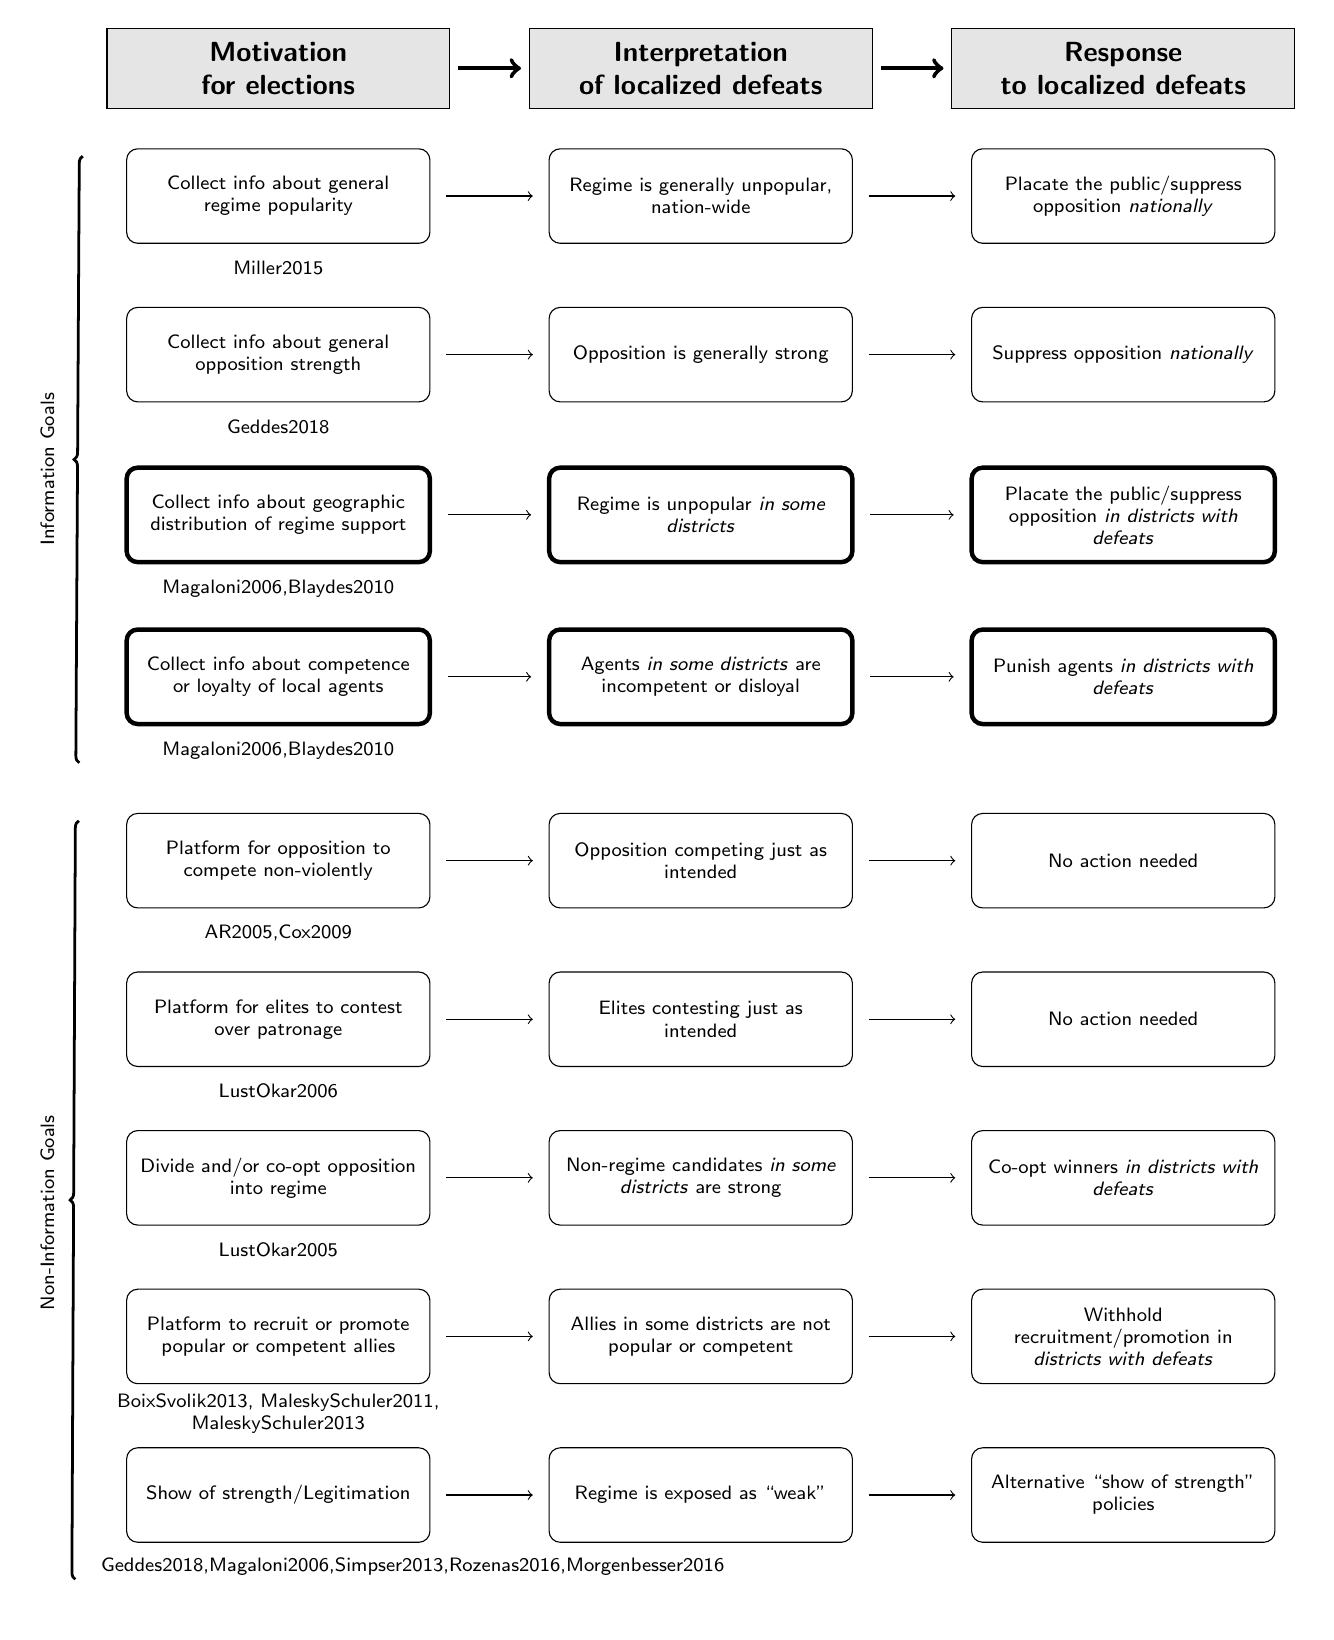
\begin{tikzpicture}
[node distance = 1cm, auto,font=\footnotesize,
% STYLES
every node/.style={node distance=3cm},
% The title style is used to draw the main title
title/.style={rectangle, draw, fill=black!10, inner sep=5pt, text width=4cm, text badly centered, minimum height=1cm, font=\bfseries\footnotesize\sffamily},
% The subtitle style is used to draw the title below main title
subtitle/.style={rectangle, inner sep= 2pt, minimum height=.5cm, node distance=0.25cm, text width=4.5cm, text badly centered, font=\scriptsize\sffamily},
% The theory style is used to draw nodes for each theory
theory/.style={rectangle, rounded corners, draw, minimum height=1.2cm, inner sep= 5pt, text width=3.5cm, node distance=0.25cm, text badly centered, font=\scriptsize\sffamily}]

%%%% Top nodes %%%%
\node [title] (interpretation) {Interpretation\\of localized defeats};
\node [title, left=1cm of interpretation] (intention) {Motivation\\for elections};
\node [title, right=1cm of interpretation] (response) {Response\\to localized defeats};

%% Top nodes subtitle

% Intention
%\node [subtitle, below=0.2cm of intention] (sub-intention) {for\\
%	authoritarian elections};

% Interpretation
%\node [subtitle, below=0.2cm of interpretation] (sub-interpretation) {of\\
%	localized defeats};

% Response
%\node [subtitle, below=0.2cm of response] (sub-response) {to\\
%	localized defeats};

%%%% Theory nodes %%%%
% B1
\node [theory, below=0.5cm of intention] (B1-intention) {Collect info about general regime popularity};
\node [subtitle, below=0.05cm of B1-intention] (B1-sub-intention) {\citep{Miller2015}};

\node [theory, below=0.5cm of interpretation] (B1-interpretation) {Regime is generally unpopular, nation-wide};
\node [subtitle, below=0.05cm of B1-interpretation] (B1-sub-interpretation) {};

\node [theory, below=0.5cm of response] (B1-response) {Placate the public/suppress opposition \textsl{nationally}};
\node [subtitle, below=0.05cm of B1-response] (B1-sub-response) {};

% B2
\node [theory, below=0.8cm of B1-intention] (B2-intention) {Collect info about general opposition strength};
\node [subtitle, below=0.05cm of B2-intention] (B2-sub-intention) {\citep{Geddes2018}};

\node [theory, below=0.8cm of B1-interpretation] (B2-interpretation) {Opposition is generally strong};
\node [subtitle, below=0.05cm of B2-interpretation] (B2-sub-interpretation) {};

\node [theory, below=0.8cm of B1-response] (B2-response) {Suppress opposition \textsl{nationally}};
\node [subtitle, below=0.05cm of B2-response] (B2-sub-response) {};

% B3
\node [theory, below=0.8cm of B2-intention, ultra thick] (B3-intention) {Collect info about geographic distribution of regime support};
\node [subtitle, below=0.05cm of B3-intention] (B3-sub-intention) {\citep{Magaloni2006,Blaydes2010}};

\node [theory, below=0.8cm of B2-interpretation, ultra thick] (B3-interpretation) {Regime is unpopular \textsl{in some districts}};
\node [subtitle, below=0.05cm of B3-interpretation] (B3-sub-interpretation) {};

\node [theory, below=0.8cm of B2-response, ultra thick] (B3-response) {Placate the public/suppress opposition \textsl{in districts with defeats}};
\node [subtitle, below=0.05cm of B3-response] (B3-sub-response) {};

% B4
\node [theory, below=0.8cm of B3-intention, ultra thick] (B4-intention) {Collect info about competence or loyalty of local agents};
\node [subtitle, below=0.05cm of B4-intention] (B4-sub-intention) {\citep{Magaloni2006,Blaydes2010}};

\node [theory, below=0.8cm of B3-interpretation, ultra thick] (B4-interpretation) {Agents \textsl{in some districts} are incompetent or disloyal};
\node [subtitle, below=0.05cm of B4-interpretation] (B4-sub-interpretation) {};

\node [theory, below=0.8cm of B3-response, ultra thick] (B4-response) {Punish agents \textsl{in districts with defeats}};
\node [subtitle, below=0.05cm of B4-response] (B4-sub-response) {};

% A1
\node [theory, below=1.1cm of B4-intention] (A1-intention) {Platform for opposition to compete non-violently};
\node [subtitle, below=0.05cm of A1-intention] (A1-sub-intention) {\citep{AR2005,Cox2009}};

\node [theory, below=1.1cm of B4-interpretation] (A1-interpretation) {Opposition competing just as intended};
\node [subtitle, below=0.05cm of A1-interpretation] (A1-sub-interpretation) {};

\node [theory, below=1.1cm of B4-response] (A1-response) {No action needed};
\node [subtitle, below=0.05cm of A1-response] (A1-sub-response) {};

% A2
\node [theory, below=0.8cm of A1-intention] (A2-intention) {Platform for elites to contest over patronage};
\node [subtitle, below=0.05cm of A2-intention] (A2-sub-intention) {\citep{LustOkar2006}};

\node [theory, below=0.8cm of A1-interpretation] (A2-interpretation) {Elites contesting just as intended};
\node [subtitle, below=0.05cm of A2-interpretation] (A2-sub-interpretation) {};

\node [theory, below=0.8cm of A1-response] (A2-response) {No action needed};
\node [subtitle, below=0.05cm of A2-response] (A2-sub-response) {};

% C1
\node [theory, below=0.8cm of A2-intention] (C1-intention) {Divide and/or co-opt opposition into regime};
\node [subtitle, below=0.05cm of C1-intention] (C1-sub-intention) {\citep{LustOkar2005}};

\node [theory, below=0.8cm of A2-interpretation] (C1-interpretation) {Non-regime candidates \textsl{in some districts} are strong};
\node [subtitle, below=0.05cm of C1-interpretation] (C1-sub-interpretation) {};

\node [theory, below=0.8cm of A2-response] (C1-response) {Co-opt winners \textsl{in districts with defeats}};
\node [subtitle, below=0.05cm of C1-response] (C1-sub-response) {};

% C2
\node [theory, below=0.8cm of C1-intention] (C2-intention) {Platform to recruit or promote popular or competent allies};
\node [subtitle, below=0.05cm of C2-intention] (C2-sub-intention) {\citep{BoixSvolik2013, MaleskySchuler2011, MaleskySchuler2013}};

\node [theory, below=0.8cm of C1-interpretation] (C2-interpretation) {Allies in some districts are not popular or competent};
\node [subtitle, below=0.05cm of C2-interpretation] (C2-sub-interpretation) {};

\node [theory, below=0.8cm of C1-response] (C2-response) {Withhold recruitment/promotion in \textit{districts with defeats}};
\node [subtitle, below=0.05cm of C2-response] (C2-sub-response) {};

% D1
\node [theory, below=0.8cm of C2-intention] (D1-intention) {Show of strength/Legitimation};
\node [subtitle, below=0.05cm of D1-intention] (D1-sub-intention) {\citep{Geddes2018,Magaloni2006,Simpser2013,Rozenas2016,Morgenbesser2016}};

\node [theory, below=0.8cm of C2-interpretation] (D1-interpretation) {Regime is exposed as ``weak''};
\node [subtitle, below=0.05cm of D1-interpretation] (D1-sub-interpretation) {};

\node [theory, below=0.8cm of C2-response] (D1-response) {Alternative ``show of strength'' policies};
\node [subtitle, below=0.05cm of D1-response] (D1-sub-response) {};

%%%% Side theory category nodes %%%%

% B
\node [subtitle, left=1cm of B1-intention.north west, rotate=90, text width = 8cm] (information) {Information Goals};

\draw [decorate,decoration=brace, line width=1pt] 
([xshift=-0.2cm, yshift=0.1cm]B4-sub-intention.south west) -- ([xshift=-0.55cm, yshift=-0.1cm]B1-intention.north west);

% A, C and D together
\node [subtitle, left=1cm of A1-intention.north west, rotate=90, text width = 10cm] (non-information) {Non-Information Goals};

\draw [decorate,decoration=brace, line width=1pt] 
([xshift=-0.25cm, yshift=0.1cm]D1-sub-intention.south west) -- ([xshift=-0.6cm, yshift=-0.1cm]A1-intention.north west);

%% A
%\node [subtitle, left=0.6cm of A1-intention.north west, rotate=90, text width = 4.4cm] (power-sharing) {``Platform''/``Power-sharing''};
%
%\draw [decorate,decoration=brace, line width=1pt] 
%([xshift=-0.2cm, yshift=0.1cm]A2-sub-intention.south west) -- ([xshift=-0.2cm, yshift=-0.1cm]A1-intention.north west);
%
%% C
%\node [subtitle, left=0.6cm of C1-intention.north west, rotate=90, text width = 1.9cm] (co-optation) {``Co-optation''};
%
%\draw [decorate,decoration=brace, line width=1pt] 
%([xshift=-0.2cm, yshift=0.1cm]C2-sub-intention.south west) -- ([xshift=-0.2cm, yshift=-0.1cm]C1-intention.north west);
%
%% D
%\node [subtitle, left=0.6cm of D1-intention.north west, rotate=90, text width = 2cm] (show-of-strength) {``Demonstration''};
%
%\draw [decorate,decoration=brace, line width=1pt] 
%([xshift=-0.2cm, yshift=0.1cm]D1-sub-intention.south west) -- ([xshift=-0.2cm, yshift=-0.1cm]D1-intention.north west);


%%%%%%%%%%%%%%%%

% Draw the links between forces
\path[->,ultra thick, shorten >=.1cm, shorten <=.1cm] 
(intention) edge (interpretation)
(interpretation) edge (response);

\path[->, shorten >=.2cm, shorten <=.2cm] 
(A1-intention) edge (A1-interpretation)
(A1-interpretation) edge (A1-response);

\path[->, shorten >=.2cm, shorten <=.2cm] 
(A2-intention) edge (A2-interpretation)
(A2-interpretation) edge (A2-response);

\path[->, shorten >=.2cm, shorten <=.2cm] 
(B1-intention) edge (B1-interpretation)
(B1-interpretation) edge (B1-response);

\path[->, shorten >=.2cm, shorten <=.2cm] 
(B2-intention) edge (B2-interpretation)
(B2-interpretation) edge (B2-response);

\path[->, shorten >=.2cm, shorten <=.2cm] 
(B3-intention) edge (B3-interpretation)
(B3-interpretation) edge (B3-response);

\path[->, shorten >=.2cm, shorten <=.2cm] 
(B4-intention) edge (B4-interpretation)
(B4-interpretation) edge (B4-response);

\path[->, shorten >=.2cm, shorten <=.2cm] 
(C1-intention) edge (C1-interpretation)
(C1-interpretation) edge (C1-response);

\path[->, shorten >=.2cm, shorten <=.2cm] 
(C2-intention) edge (C2-interpretation)
(C2-interpretation) edge (C2-response);

\path[->, shorten >=.2cm, shorten <=.2cm] 
(D1-intention) edge (D1-interpretation)
(D1-interpretation) edge (D1-response);


\end{tikzpicture} 
\caption{Key theories of authoritarian elections and their predictions about how regime leaders perceive and respond to localized defeats. Two theories most relevant to the Vietnam case are highlighted with bold borders.}
\label{fig:Theory}
\end{figure}

}

\subsection*{The CPV's Response to Central Candidate Defeats}
\label{sec:vietnam_local_defeat}

In the case of Vietnam, the CPV's response to the defeats of central candidates in the VNA elections is especially useful in identifying how the party perceived these defeats and consequently what informational goal it had for these elections. The reason is that, due to the highly institutionalized and structured nature of Vietnamese politics, the scope of possible post-election actions that the CPV could take is so limited that it would not be able to react to all the incoming information without one reaction compromising the effect of another.

In particular, whereas most high-level policy instruments in Vietnam are inflexible, requiring debate and ratification by the VNA or the CPV's Central Committee, the central party leadership can rely on annual budgetary allocations in managing their relationships with both the public and local governments. Each province's share of the national budget is calculated based on its projected revenues and expenditures. Provincial revenues fall into two categories--revenues provinces always get to keep, and revenues they may have to share with the central government according to pre-determined sharing rates \parencite[for more details, see][]{MartinezVazquez2004}. Most provinces expect more expenditures than revenues and get to keep the shared revenues. In addition, the central government provides for equalization grants to provinces that cannot cover their expenditures even with the shared revenues, as well as other conditional or targeted transfers. Because most provinces spend more money than they can raise, these various forms of central transfers become indispensable for local governance. The remaining provinces are net-contributors to the budget, meaning that they send back to Hanoi more than they receive in transfers.

%Decisions about central transfers result from an opaque but regular negotiation process. Every year, individual provinces begin this process by submitting to the central government their budget plans, which include revenue and expenditure forecasts. The central government negotiates these numbers with each province until an agreement is reached, at which point the provinces' numbers are integrated into a national budget to be rubber-stamped by the VNA.
Decisions about central transfers result from an opaque but regular negotiation process. Every year, each province must submit its revenue and expenditure forecasts to the central government and negotiates both numbers until an agreement is reached. Meanwhile, the sharing rates for shared revenues are fixed for cycles of every three to five years to make provincial revenues more predictable. (Not coincidentally, these ``budget-stability periods'' begin only after an election year, and extend until just before the next election.)
 %\fnote{The election timing in turn follows the timing of the National Party Congress.} 
This means that the regime has two opportunities to influence central transfers to individual provinces: one right after each election (when they negotiate fixed components of the budget) and one every year after (when they determine other types of transfers by fixing expected revenues and expenditures). Different considerations may motivate central transfer adjustments, one of which could be new information from election results.

Two of the hypotheses about post-election responses to localized defeats in \autoref{fig:Theory} predict diametrically opposite adjustments to central transfers by the CPV. Specifically, if the regime intends to use VNA elections to measure the distribution of regime popularity, it will see central candidate defeats as indicators for provinces with faltering public support. The appropriate reaction to this information would be to give the public some concession, which would require an \textit{increase} in central transfers to those provinces. By increasing central transfers, the party enables the provinces to invest in public goods, which is a straightforward way to bolster regime support.\fnote{In theory, this strategy may create perverse incentive for citizens to keep voting against central candidates. In practice, successful strategic voting requires an unfeasible level of citizen coordination. See Online Appendix \ref{app:repeat} for further discussion and empirical evidence.}

However, if the CPV uses elections to evaluate province-level officials, the defeats will reveal the identity of executives who are too incompetent or too independent. In this case, the CPV should punish the officials in question. However, because explicit methods of punishment, like firing, demotion, or withholding promotion require several institutional hurdles and broadcast negative signals about the regime's internal unity, the CPV rarely uses them except for serious transgressions. Instead, it can carry out more subtle but targeted punishments of local officials with a \textit{decrease} in central transfers.\fnote{In Online Appendix \ref{app:punishment}, I show that the CPV did not issue explicit punishment to officials in provinces that experienced central candidate defeats in 2007, 2011, and 2016.} As with many other authoritarian regimes, in Vietnam corruption opportunity serves as a form of compensation for lower-level officials \citep{Darden2008}. Cutting central transfers reduces the scope for corruption and directly affects their income. In addition, it also limits these officials' power by reducing their ability to distribute rent further downward.

For changes in central transfers to reveal the CPV's interpretation of central candidate defeats, it is not necessary for budget adjustments to serve as the primary policy instrument for placating the public or punishing regime agents. As long as each goal requires central transfers to be adjusted in a different direction, observing the direction in which central transfers are adjusted will reveal the CPV's preference. Indeed, increasing central transfers would help appease the public, but because provincial officials have the \textit{de facto} control over how central funds are allocated once they have been approved, the CPV has little interest in doing so if it believes that these officials are disloyal or incompetent, in which case the funding would simply be used inefficiently, get embezzled, or even create perverse incentives in future elections. Similarly, decreasing central transfers would punish provincial executives but also deepen resentment among citizens, meaning that the CPV will only do so if it does not worry about the local level of regime support. In other words, evidence that the CPV altered the flow of transfers to provinces with central candidate defeats in any direction would be sufficient to confirm that it had chosen to listen to one signal and ignore the other.

\section*{Empirical Design}
\label{sec:methods}

To analyze whether the CPV increased or decreased central transfers to provinces where localized defeats had happened, I apply several panel data methods to identify the defeats' effect on central transfers. I make use of the most comprehensive dataset on budgetary allocations in Vietnam to date--which was made possible by the government's inauguration in September 2020 of a new online portal to publicize budget documents at the national and provincial levels. I focus on central transfer changes around the recent VNA elections in April 2016, when 16 out of 197 central candidates suffered defeats in seven out of 63 provinces. The 2016 election offers an unprecedented opportunity to conduct such an analysis for two main reasons. First, because budget data for Vietnam is only available from 2004 onward, focusing on the most recent election ensures a sufficient number of pre-treatment periods for panel data methods. Second, the CPV has only released vote shares for defeated candidates starting from the 2016 election. Complete vote share data is required to identify central candidates whose victories and defeats were narrow enough to be plausibly considered as similar to each other, which helps maximize the internal validity of this analysis.

\subsection*{Identifying Close Defeats and Victories}
\label{sec:methods_sample}

To identify the true effects of the CPV's response to localized defeats, ``treated'' provinces (which experienced localized defeats) need to be compared against ``control'' provinces (which did not experience such defeats) that are similar in every other regard. However, these two sets of provinces may differ significantly from each other. 
%\citet{MaleskySchuler2011} already show that provinces with these defeats tend to be more financially independent. If this paper's theory is correct, they may also have dissatisfied voters or low-quality executives. At the candidate level, some races are also different from others: provinces in which the regime's top leaders contest, is undoubtedly less likely to see these defeats.
Drawing upon insights from the matching methods and the regression discontinuity design, I prune the sample of incomparable cases by limiting it to close races in which the central candidate narrowly lost or won. I achieve this with two separate approaches. First, at the province level, I select only provinces in which at least one central candidate won or lost with a margin smaller than 10 percentage points--a margin that the CPV officially considers to be low \citep{MaleskySchuler2011}.

The second approach seeks to achieve as-if randomization at the candidate level. Following \citet{CattaneoTitiunik2015}, I conduct a grid search to identify the upper and lower vote margin boundaries that would produce the largest window within which central candidates who lost and who won are statistically indistinguishable in terms of all pre-treatment candidate-level and district-level characteristics.\fnote{Specifically, I increment each boundary by $0.25$ at a time to generate a grid of possible windows. For each window, I test the sharp null hypothesis of no treatment effects on each of the chosen characteristics using the ATE test statistic, and reject any window for which any of these tests has a p-value of above 0.15. The candidate-level characteristics are age, gender, party membership, party history, education, political power--operationalized following \citet{MaleskySchuler2011}, and the district-level characteristics are number of candidates and number of seats.} The resulting window is found to be $(-11.25, 7.75)$. Since the fates of central candidates whose vote shares fell within this window can be assumed to be as-if random, it is possible to conduct inference through independent re-randomization. 

For both approaches, I drop two clear outliers--the capital Hanoi and the biggest municipality Ho Chi Minh City. While the central government also considers election results when adjusting central transfers to these provinces, many other governance goals uniquely pertaining to these mega-cities also pull transfers in various directions. Because the Party Secretaries of Hanoi and Ho Chi Minh City both sit in the Politburo--the highest echelon of leadership within the CPV--the availability of information, channels for getting state resources and modes of accountability in these two provinces are also incomparable to all the other provinces. Finally, I also exclude the province of Binh Duong, which experienced a major change in budget allocation in 2017 following the introduction of a revised State Budget Law \citep{BaoViet2016}.

These two approaches produce the same set of treated provinces but arrive at two slightly different sets of control provinces. Table \ref{tab:balance} shows the balance between control and treated provinces across several relevant covariates, all of which are measured in 2015. For both samples, the difference between treatment and control means is subjected to both a randomization-inference and a standard OLS hypothesis test. The results show that the treated and control provinces in the first sample are nearly identical. The second sample, even though constructed to achieve balance only at the candidate and district levels, also displays balance when aggregated to the province level. 

\afterpage{%

\begin{landscape}\begin{table}[!h]

\caption{\label{tab:balance}Balance between control and treatment provinces based on 2015 data}
\centering
\resizebox{\linewidth}{!}{
\begin{tabular}[t]{>{\raggedright\arraybackslash}p{14em}>{\raggedleft\arraybackslash}p{4.1em}>{\raggedleft\arraybackslash}p{4.1em}>{\centering\arraybackslash}p{4.1em}>{\centering\arraybackslash}p{4.1em}>{\centering\arraybackslash}p{4.1em}>{\raggedleft\arraybackslash}p{4.1em}>{\raggedleft\arraybackslash}p{4.1em}>{\centering\arraybackslash}p{4.1em}>{\centering\arraybackslash}p{4.1em}>{\centering\arraybackslash}p{4.1em}}
\toprule
\multicolumn{1}{c}{ } & \multicolumn{5}{c}{Linear Fixed Effects Sample} & \multicolumn{5}{c}{Local Randomization RDD Sample} \\
\cmidrule(l{3pt}r{3pt}){2-6} \cmidrule(l{3pt}r{3pt}){7-11}
\multicolumn{1}{>{\centering\arraybackslash}p{14em}}{ } & \multicolumn{1}{>{\centering\arraybackslash}p{4.1em}}{Control Mean ($N = 9$)} & \multicolumn{1}{>{\centering\arraybackslash}p{4.1em}}{Treated Mean ($N = 4$)} & \multicolumn{1}{>{\centering\arraybackslash}p{4.1em}}{Std. Diff. in Means} & \multicolumn{1}{>{\centering\arraybackslash}p{4.1em}}{RI p-value} & \multicolumn{1}{>{\centering\arraybackslash}p{4.1em}}{OLS p-value} & \multicolumn{1}{>{\centering\arraybackslash}p{4.1em}}{Control Mean ($N = 11$)} & \multicolumn{1}{>{\centering\arraybackslash}p{4.1em}}{Treated Mean ($N = 4$)} & \multicolumn{1}{>{\centering\arraybackslash}p{4.1em}}{Std. Diff. in Means} & \multicolumn{1}{>{\centering\arraybackslash}p{4.1em}}{RI p-value} & \multicolumn{1}{>{\centering\arraybackslash}p{4.1em}}{OLS p-value}\\
\midrule
\addlinespace[0.3em]
\multicolumn{11}{l}{\textbf{Budget}}\\
\hspace{1em}Budget Revenue (Billions of VND) & 2871.2 & 3753.2 & 0.49 & 0.51 & 0.51 & 5576.0 & 3753.2 & -0.20 & 0.92 & 0.71\\
\hspace{1em}Budget Expenditure (Billions of VND) & 5017.6 & 4942.5 & -0.05 & 0.94 & 0.93 & 5523.6 & 4942.5 & -0.26 & 0.69 & 0.64\\
\addlinespace[0.3em]
\multicolumn{11}{l}{\textbf{Election}}\\
\hspace{1em}Number of Seats & 7.4 & 6.8 & -0.60 & 0.46 & 0.31 & 7.5 & 6.8 & -0.71 & 0.16 & 0.23\\
\hspace{1em}Number of Candidates & 13.2 & 11.8 & -0.77 & 0.30 & 0.23 & 13.4 & 11.8 & -0.87 & 0.13 & 0.17\\
\hspace{1em}Number of Central Candidates & 3.1 & 2.5 & -0.81 & 0.33 & 0.17 & 3.2 & 2.5 & -0.91 & 0.07 & 0.13\\
\addlinespace[0.3em]
\multicolumn{11}{l}{\textbf{Structural Condition}}\\
\hspace{1em}Surface Area (Thousands Km$^2$) & 4579.9 & 3047.4 & -0.47 & 0.35 & 0.39 & 4408.5 & 3047.4 & -0.44 & 0.42 & 0.43\\
\hspace{1em}Population (Thousands) & 1277.3 & 1215.1 & -0.13 & 0.80 & 0.82 & 1338.2 & 1215.1 & -0.24 & 0.64 & 0.67\\
\hspace{1em}Population Density (Thousands/Km$^2$) & 399.3 & 500.8 & 0.31 & 0.58 & 0.60 & 428.7 & 500.8 & 0.22 & 0.68 & 0.70\\
\addlinespace[0.3em]
\multicolumn{11}{l}{\textbf{Economic}}\\
\hspace{1em}Provincial GDP (Billions of VND) & 44646.2 & 43129.7 & -0.08 & 0.88 & 0.90 & 58482.0 & 43129.7 & -0.31 & 0.64 & 0.56\\
\hspace{1em}Average Monthly Income (Thousands of VND) & 2083.9 & 2221.0 & 0.33 & 0.59 & 0.56 & 2237.1 & 2221.0 & -0.03 & 0.96 & 0.96\\
\hspace{1em}Employment Rate Among >15yo Population ($\%$) & 59.9 & 57.5 & -0.48 & 0.38 & 0.39 & 60.2 & 57.5 & -0.56 & 0.30 & 0.32\\
\hspace{1em}Share of Agriculture Land ($\%$) & 46.8 & 62.2 & 0.71 & 0.23 & 0.25 & 49.1 & 62.2 & 0.60 & 0.31 & 0.33\\
\addlinespace[0.3em]
\multicolumn{11}{l}{\textbf{Public Goods}}\\
\hspace{1em}Infant (<5yo) Mortality Rate (\textperthousand) & 22.8 & 18.2 & -0.40 & 0.56 & 0.46 & 22.0 & 18.2 & -0.33 & 0.68 & 0.54\\
\hspace{1em}Number of Beds in Public Hospitals & 3566.8 & 3442.2 & -0.12 & 0.89 & 0.87 & 3516.1 & 3442.2 & -0.07 & 0.93 & 0.92\\
\hspace{1em}Number of Schools & 435.3 & 359.8 & -0.55 & 0.36 & 0.34 & 418.5 & 359.8 & -0.42 & 0.50 & 0.46\\
\hspace{1em}Number of Primary Schools & 244.8 & 220.5 & -0.28 & 0.65 & 0.63 & 235.7 & 220.5 & -0.17 & 0.79 & 0.76\\
\bottomrule
\end{tabular}}
\end{table}
\end{landscape}

}

Analyses that use close elections often face two problems, but neither is detrimental in this case. First, in a sample of only close elections, defeats certainly convey a weaker signal, and are thus less likely to elicit a detectable response. While this is true, the exact closeness of each result is not necessarily apparent to the regime when there are multiple candidates in a race. In contrast, a defeat by any margin still presents an obvious personnel challenge to the regime and attracts attention from the public. This means that the binary signal of a defeat should still convey much, if not most, of a result's informational value.
%In addition, because both samples keep all but one of the central candidate defeats, any potential bias can only arise from not using large victories as the basis of comparison, which should only work against any finding.
Second, the local nature of this approach may limit its generalizability, particularly if only the weakest central candidates would be found in closely winning or losing elections. However, most central candidates are quite homogeneous in reality, and those whose vote margins are close do not differ much from those who have won more comfortably. As Table \ref{tab:candidates_stats} in Online Appendix \ref{app:bandwidth} shows, even though candidates in close elections do seem to have slightly weaker backgrounds, the difference is substantively small.

%Whereas limiting the analysis to close elections helps achieve balance between treated and control provinces and thus enhances my analyses' internal validity, it also introduces serious external validity concerns. First, races that were lost or won narrowly may be very different from most other races that include a central candidate. Specifically, central candidates who are in a position to only win narrowly may be weaker than average, or may have been sent to provinces that are more difficult than average. Second, if the central candidate defeats in the sample are so close that they could have been generated by chance, which means that the information content from these results may be weaker than that from heavy defeats.
%
%Both these concerns arise from the fact that limiting the sample leads to analyses that are inherently local in nature \citep{SkovronTitiunik2015}, but one that is seen as necessary for valid causal inferences \citep{Imbens2010}. They are particularly serious in this situation because the sample that will be used in the final analysis will comprise only a small portion of the population (13 or 15 provinces, out of all the 63 provinces in Vietnam).
%
%Some theoretical and empirical considerations may ameliorate these concerns. First, even weaker central candidates are still important regime elites who have survived the three negotiation rounds, and their defeats still disrupt personnel decisions in the future VNA while also being observed by every member of the public. Even if the regime was comparatively willing to tolerate these close defeats, it certainly did not expect them to happen, and definitely did not know ahead of time which candidate was going to lose. The defeats therefore still conveyed important information to the regime. Second, if the signal from close defeats have indeed been weaker, then any treatment effect estimate would be a conservative estimate of the regime's reaction to heavier and thus more informative losses. 
%
%Third, most central candidates do not seem to differ much from those in close races. While a small number of central candidates were indeed the regime's very top leaders and stand out in many dimensions, the majority of central candidates--144 out of 197--were similar to those selected to be in the sample, in that they were all nominated either by the VNA or the VFF blocs. Table \ref{tab:candidates_stats} in Online Appendix \ref{app:bandwidth} also shows that they are not quantitatively different. 
%
%Fourth, the above procedures only drop one out of five treated provinces for being too lopsided, but Online Appendix \ref{app:small_sample} shows that when it is added back in--such that the treatment effect estimates identify the effect of all central candidate defeats outside of Hanoi and Ho Chi Minh City--the results do not seem to change. Similarly, expanding the boundaries also introduces no significant change to the treatment effects, suggesting that the estimated local effects may indeed be generalizable.
	

\subsection*{Estimation Methods}
\label{sec:methods_estimation}

For the main analysis, I employ three different estimation and inference methods. First, I apply a linear fixed effects model to the province-level sample:
\begin{equation}
\Delta Y_{it} = \beta D_{it} + \omega T_{i} + \gamma X_{it} + \lambda_i + \delta_t + \epsilon_{it} \label{eq:FE}
\end{equation}
where $\Delta Y_{it}$ is the (neg)log of the first difference in net central transfers for province $i$ at time $t$ i.e. $\Delta Y_{it} = \log(Y_{it} - Y_{i, t-1})$ and $X_{it}$ is a vector of time-varying covariates. $T_{i}$ takes the value of 1 for every province that experienced localized defeat in 2016 and 0 otherwise, and does so for every year in the sample. Depending on whether the model seeks to estimate the \textit{instantaneous} effect that manifests in the year after or the \textit{persistent} effect that arises so in all post-election years, $D_{it} = T_{i}$ for $t=2017$ or $t\geq2017$, and is  $0$ otherwise. %\fnote{$D_{it}$ is ``lagged'' by one year for the fact that budget allocation decisions are made at the beginning of each year, such that the effect of the 2016 election only begins to manifest in 2017.} 
Here, $\lambda_i$ and $\delta_t$ are province and time fixed effects. For all analyses, $t \in \{2012, \ldots, 2019\}$ to exclude the years before the previous election.

Whereas standard fixed effects models are a generalization of the difference-in-difference framework, the use of the first-differenced outcome here generalizes my model to the triple differences method. Specifically, by allowing potential outcomes to be framed in terms of changes compared to previous years, the model can account for differences in pre-treatment trends across treated and control provinces. It also relaxes the assumption of parallel trends to one of linear trends.
%This is because whereas the standard difference-in-difference compares difference in pre- and post-treatment means across treatment groups, my model would also subtract away from this difference the year-to-year changes in outcomes, which may be different for each group. It thus relaxes the assumption of parallel trends to one of linear trends.

Second, I use the candidate-level sample to conduct a regression discontinuity analysis via the local randomization approach by \citet{CattaneoTitiunik2015}. The reasoning is as follows: for a small enough window around the treatment assignment threshold, any unit's observed treatment status can be considered as-if random. This interpretation allows for exact randomization-based inference methods that are more appropriate for small samples. Specifically, I use independent coin flips to re-randomize $10,000$ times the election outcome of every central candidate in the sample, aggregate the result to the province level, estimate new treatment effects using the same linear fixed effects model as above, and then compare the distribution of these re-randomized effects with the observed effect.

Finally, to eliminate the problem of dynamic causality \citep{ImaiKim2019}, 
%which arises out of the interdependence between central transfers in pre-election years (past outcomes), central transfers in post-election years (future outcomes), and election results (treatment), 
I also implement a generalized synthetic control analysis \citep{Xu2017gsynth}. This method uses data from control units and an interactive fixed effects model with $r$ orthogonal time-varying shocks (where $r$ is selected by cross-validation) to estimate for each treated unit a synthetic control that matches it in terms of all pre-treatment outcomes. This helps neutralize the effect of any imbalance in covariates, in past treatment or in past outcomes, leaving the treatment assignment as the only difference between each treated unit and its synthetic control. For each treated unit, the difference in post-treatment outcomes when compared to the synthetic control identifies an individual treatment effect. Because this method's performance increases with the number of pre-treatment periods, I use the entire panel of available data from 2003 to 2019, but also explicitly control for each province's past defeats. To make more data available to estimate the synthetic controls, I relax the province-level sample to include 11 additional provinces with close central candidate victories in previous elections.

\section*{Results}
\label{sec:results}

Excluding Hanoi and Ho Chi Minh City, five provinces saw one or more central candidate defeats in the 2016 election: Can Tho, Dong Thap, Phu Yen, Soc Trang and Tra Vinh. On average, each received 2 trillion VND ($86.7$ million USD) more in central transfers in 2017 than the other provinces. A naive randomization inference procedure finds that this effect is larger than 69\% of those observed under random assignments of localized defeats. Individually, \textit{all} five provinces experienced an upward change either to the level or the over-time trajectory of central transfers.

%Looking at individual provinces, the largest increase in central transfers was in Tra Vinh, where an increase of 920 billion VND (approx. $39.9$ million USD) in 2017 brought the average level of net transfers in the three post-election years to 3,410 billion VND per year (approx. $147.8$ million USD), compared to the average level of 2,560 billion VND per year (approx. $111$ million USD) in the three years preceding the election. The smallest change in transfers was in Can Tho, a net contributor to the national budget which saw its contribution burden reduced from an average of 1920 billion VND (approx. $83.3$ million USD) per year in the three pre-election years to an average of 1900 billion VND (approx. $82.4$ million USD) per year in the three post-election years, despite the economy's steady growth throughout this period. More importantly, 2017 and 2018 marked the first years Can Tho's contribution burden has decreased, after having steadily increased since 2014.

Interestingly, the consistency with which the CPV increased central transfers to these five provinces contrasts with the variation in how central candidate defeats had happened: in some provinces such as Can Tho or Soc Trang, many votes were concentrated to one particularly strong local elite, whereas in others the dissent votes spread evenly over several local candidates. 
%Even though the former pattern could have indicated a province's intention to prioritize its own candidate above all and the latter may suggest a conspiracy against the central candidate in particular, the CPV evidently increased funding to all the five provinces. 
Furthermore, it also issued no formal punishment to any of the five provinces' leaders.\fnote{Online Appendix \ref{app:qualitative} presents further details about the local dynamics in each province.} Based on this finding alone, it seems likely that Vietnam's leaders have chosen to discount local officials' responsibility for these defeats. To verify this claim, the increased transfers to provinces that experienced localized defeats must be compared against funding patterns in similar provinces that did not.


% Table created by stargazer v.5.2.2 by Marek Hlavac, Harvard University. E-mail: hlavac at fas.harvard.edu
% Date and time: Fri, Feb 12, 2021 - 2:46:41 PM
\begin{table}[!htbp] \centering 
  \caption{Estimated treatment effects of localized defeats on log of first-differenced central transfers from linear fixed effects models. Cluster-robust standard errors appear in parentheses.} 
  \label{tab:lfe_main} 
\begin{tabular}{@{\extracolsep{5pt}}lcccccc} 
\\[-1.8ex]\hline 
\hline \\[-1.8ex] 
 & \multicolumn{3}{c}{Instantaneous Effect} & \multicolumn{3}{c}{Persistent Effect} \\ 
\\[-1.8ex] & (1) & (2) & (3) & (4) & (5) & (6)\\ 
\hline \\[-1.8ex] 
 Treatment Effect & 9.093$^{**}$ & 9.104$^{*}$ & 9.093$^{**}$ & 6.366$^{***}$ & 6.552$^{**}$ & 6.366$^{***}$ \\ 
  & (4.580) & (4.684) & (4.223) & (2.246) & (2.760) & (2.125) \\ 
 \hline \\[-1.8ex] 
Election Competitiveness &  &  & Yes &  &  & Yes \\ 
Time-variant Covariates &  & Yes &  &  & Yes &  \\ 
Province FEs & Yes & Yes &  & Yes & Yes &  \\ 
Year FEs & Yes & Yes & Yes & Yes & Yes & Yes \\ 
\hline \\[-1.8ex] 
N & 70 & 70 & 70 & 98 & 98 & 98 \\ 
R$^{2}$ & 0.604 & 0.604 & 0.439 & 0.478 & 0.489 & 0.357 \\ 
\hline 
\hline \\[-1.8ex] 
\multicolumn{7}{l}{$^{*}$p $<$ .1; $^{**}$p $<$ .05; $^{***}$p $<$ .01} \\ 
\end{tabular} 
\end{table} 


Table \ref{tab:lfe_main} shows the main results from a comparison using the linear fixed effects model, under different model specifications. The treatment effect estimates are positive, significant, and stable across specifications. Since the outcome variable is the log of first-differenced net transfers, the effect magnitude is best understood as multiples of the average annual change in net transfers between non-election years. For example, following the first three columns of Table \ref{tab:lfe_main}, if net transfers to a province have been growing at an average rate of $100$ billion VND ($4.4$ million USD) per year, then a localized defeat would add $910$ billion VND ($39.8$ million USD) to the province's 2017 transfers.\fnote{Among treated provinces, annual changes in central transfers between 2012 and 2016 average to between $87$ billion in Phu Yen to $218$ billion VND in Can Tho ($3.8$ to $9.5$ million USD). The estimated effect for 2017 thus translates to about $791$ billion to $2$ trillion  VND ($34.6$ to $86.7$ million USD). In comparison, these provinces' expenditures in 2016 ranges from $3.9$ trillion in Phu Yen to $6.3$ trillion VND in Can Tho ($170.5$ to $275.4$ million USD).} Estimates for the persistent effect in the last three columns are also positive and statistically significant; their smaller values suggest that net transfers to treated provinces keeps accumulating in the post-election period but at a decreasing pace.

%\fnote{Among the provinces in the sample, Tien Giang experienced the smallest average change in net transfers--approximately $56$ billion VND ($2.4$ million USD) per year, whereas Dak Lak experienced the largest--approximately $820$ billion VND ($35$ million USD) per year. The estimated effect translates to roughly $5$ billion VND ($214,000$ USD) for Tien Giang and $75$ billion VND ($3.2$ million USD) for Dak Lak. In comparison, average total expenditure is $5,500$ billion VND ($237$ million USD) for Tien Giang and $8,470$ billion VND ($363$ million USD) for Dak Lak.} 

%\fnote{Because treatment effects are estimated for first-differenced outcomes, even though persistent effect estimates are smaller than those of the instantaneous effect, they still show that net transfers to treated provinces keeps accumulating throughout the post-election period but with a gradually decreasing pace. Figure \ref{fig:synth_placebo} provides a clearer illustration of this effect.}

To allay concerns about lack of exogeneity, Figure \ref{fig:lfe_placebo} plots the first three estimates in Table \ref{tab:lfe_main} against three placebo treatment effects for 2013, 2014, and 2015. The placebo treatment effects are estimated by moving the treatment indicators backward in time as if the election had happened earlier than it actually did. Because the election could not have affected budget allocation before it took place, the true treatment effects should be zero for these years, and any measured difference between treated and control provinces would only reflect an imbalance in the data. The results in Figure \ref{fig:lfe_placebo} reassuringly show no such difference: all placebo effects are estimated to be statistically insignificant, with the 2013 and 2015 effects being particularly close to zero.

\begin{figure}[!htbp]
	\centering
	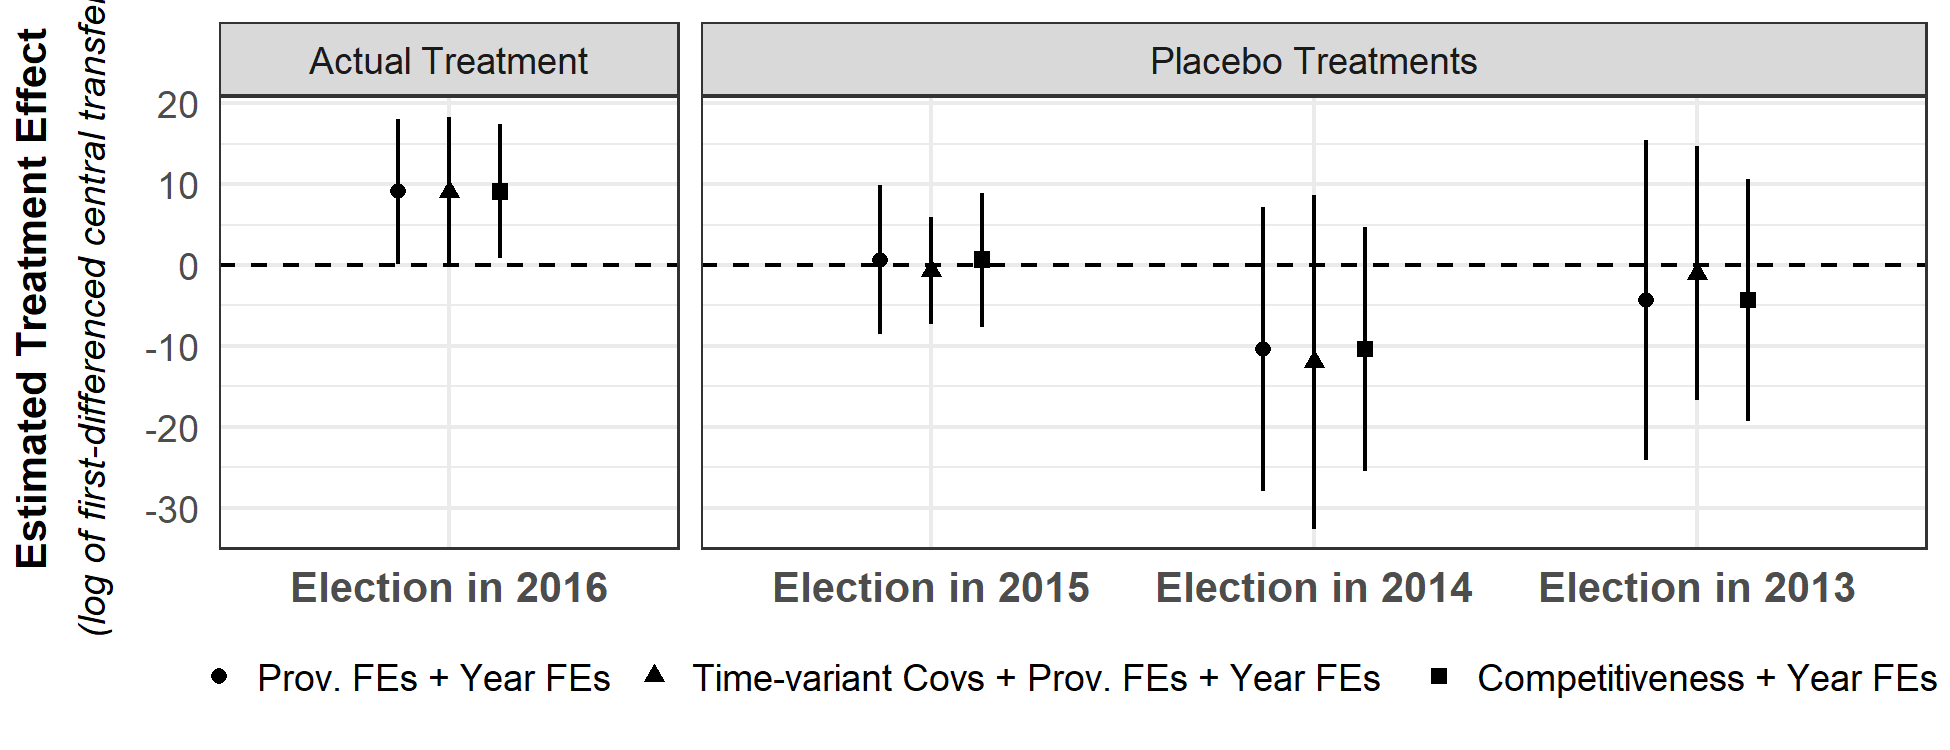
\includegraphics[]{figure/210202_lfe_placebo.png}
	\captionsetup{singlelinecheck=off}
	\caption[Estimated placebo linear fixed effects treatment effects]{Estimates of instantaneous treatment effects on log of first-differenced central transfers using linear fixed effects models. Error bars show 95\% confidence intervals.}
	\label{fig:lfe_placebo}
\end{figure}

Figure \ref{fig:rdd_placebo} presents the results from the local randomization analysis. Since this analysis does not rely on large sample asymptotics, its inferences are not subjected to the small sample concerns that may have cast doubt on the previous results. Instead, the null distribution is constructed by re-randomizing the election outcomes of each of the 17 central candidates from 15 provinces in the candidate-level sample. The treatment effect, estimated for the observed scenario where four candidates lost in four different provinces, is equivalent to an addition of about 10 times a province's annual change in central transfers, and lies far enough toward the tail end of the null distribution to be considered statistically significant. The opposite applies to the placebo results, suggesting that any imbalance between treated and untreated provinces is small and close to zero. Similar to Figure \ref{fig:lfe_placebo}, a negative but statistically insignificant difference is detected for the 2014 placebo. 

\begin{figure}[!htbp]
	\centering
	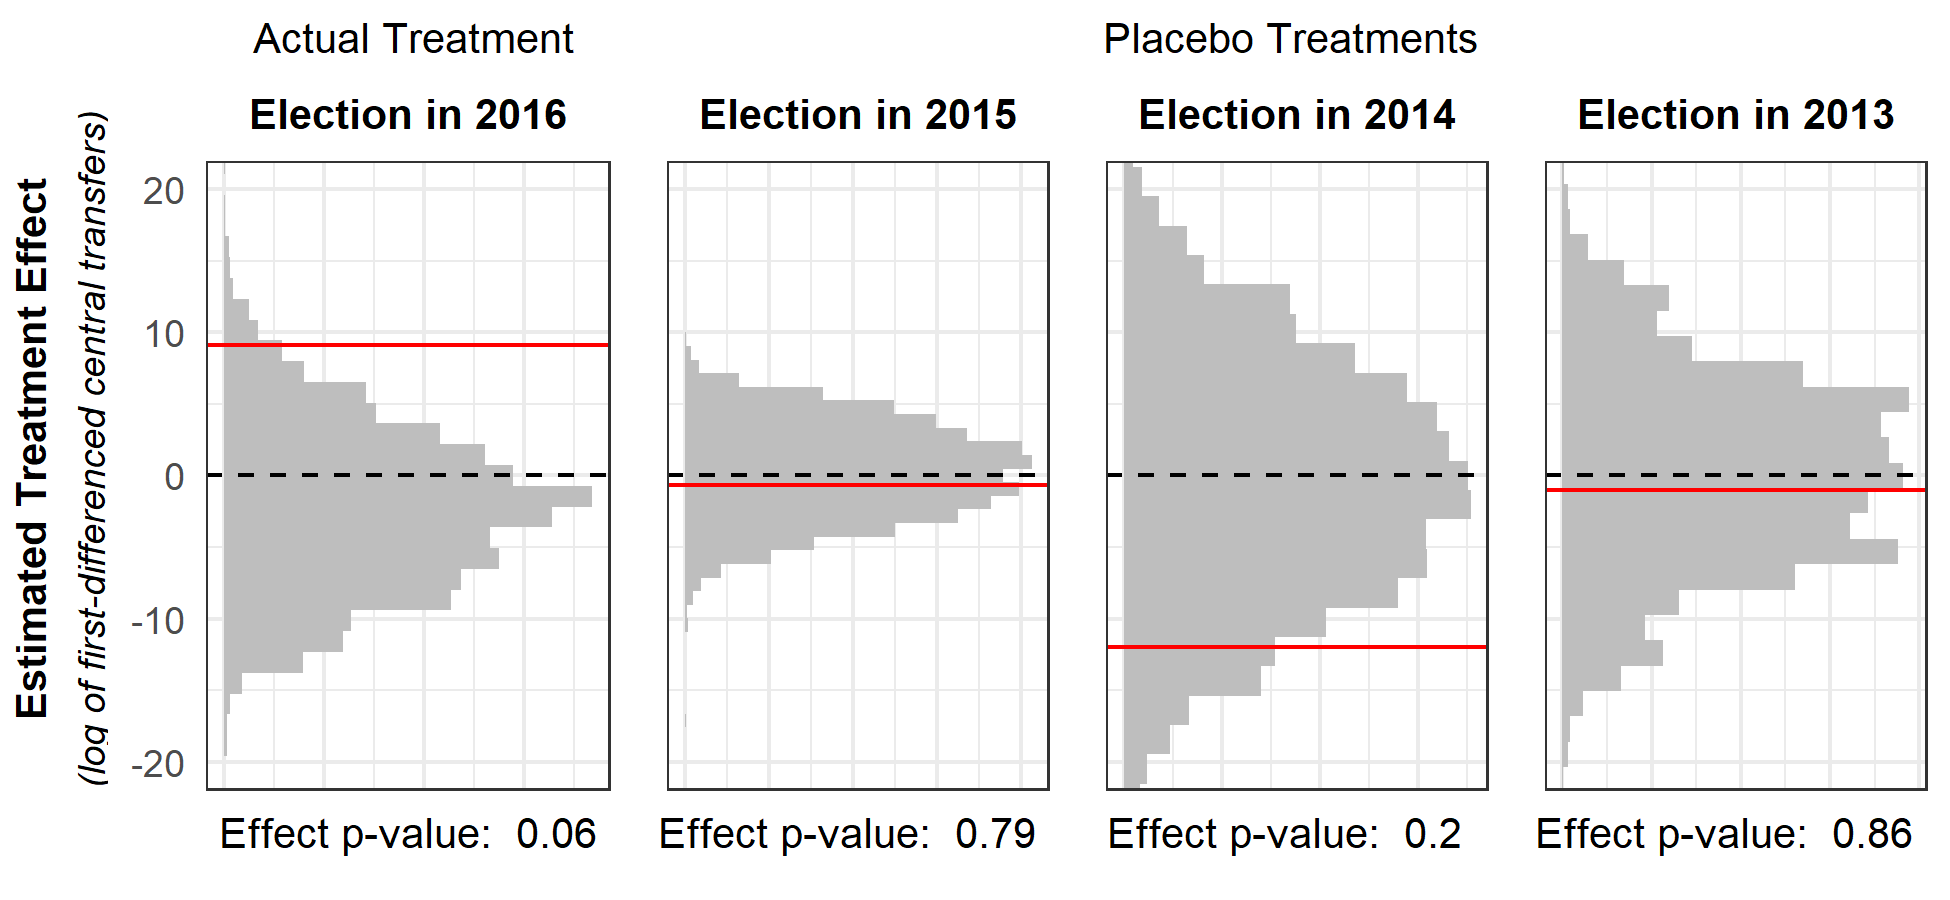
\includegraphics[]{figure/210202_rdd_results.png}
	\captionsetup{singlelinecheck=off}
	\caption[Estimated RDD treatment effects]{Estimates of instantaneous treatment effects on log of first-differenced central transfers from RDD analyses using the local randomization approach. The red lines show the estimated treatment effects, and the gray bars show their randomization distribution. P-values are presented for the treatment effect estimate.}
	\label{fig:rdd_placebo}
\end{figure}

Finally, Figure \ref{fig:synth_placebo} shows treatment effect estimates from the generalized synthetic control method averaged over all four treated provinces. Since the linearity assumption is not necessary for this method, I use logged net transfers as the outcome variable instead of its first difference. The result confirms not only a statistically significant and sustained treatment effect throughout the post-election years, but also the absence of pre-treatment difference in the years prior to the election. The latter verifies that the generalized synthetic control has eliminated dynamic causality as intended. Echoing Table \ref{tab:lfe_main}, Figure \ref{fig:synth_placebo} shows that the transfer increases were steepest in the first year after the election, but still increased albeit with plateauing slopes over the subsequent years.

\begin{figure}[!htbp]
	\centering
	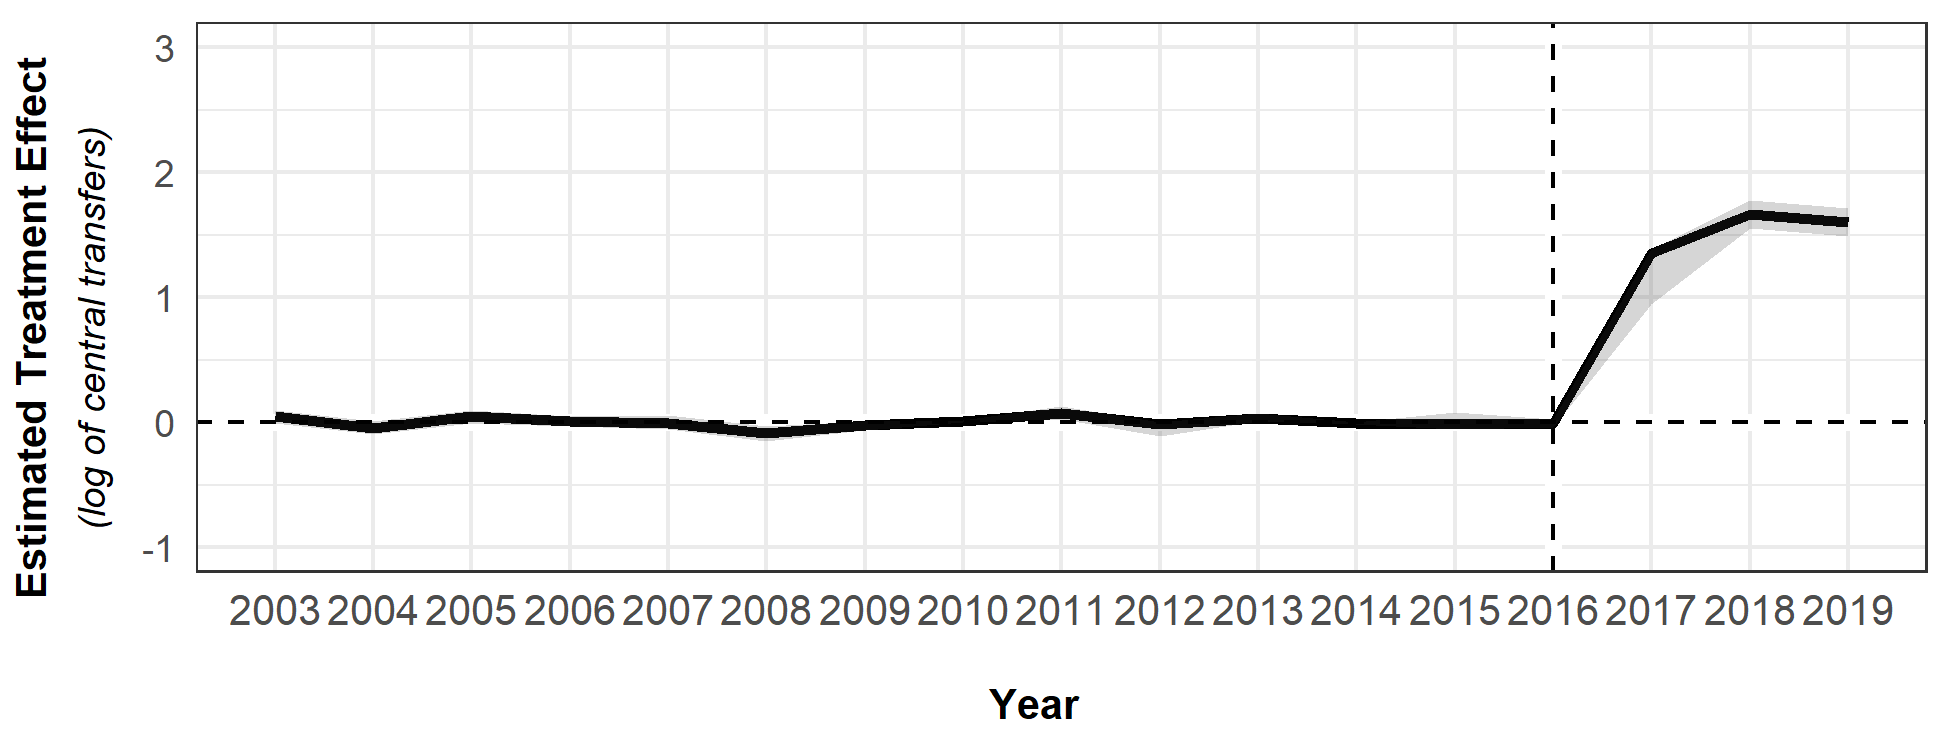
\includegraphics[]{figure/210202_synth_results.png}
	\captionsetup{singlelinecheck=off}
	\caption[Estimated synthetic control treatment effects]{Estimates of treatment effects on log of central transfers using the generalized synthetic control method. The gray region represents the 95\% confidence interval obtained by the parametric bootstrap. The vertical dashed line marks the election year.}
	\label{fig:synth_placebo}
\end{figure}

%\subsection*{Robustness of Key Results}

Altogether, the three analyses present a consistent set of findings suggesting that leaders in Vietnam increased transfers to provinces in which central candidates were defeated in the 2016 VNA election. All estimated treatment effects are statistically and substantively significant, and have survived sufficient placebo tests. They are also robust to some additional challenges:

First, even though the small sample size--particularly the number of treated provinces--may suggest a cause for concern, in Online Appendix \ref{app:small_sample} I show that it does not compromise the finding's validity. In terms of inferences, the exact tests using randomization inference are adequate because they do not depend on asymptotic properties. In terms of estimate reliability, I use a jackknife procedure that introduces perturbations to the sample by adding or dropping treatment or control provinces one at a time to generate 62 new different samples, and re-estimate the main effects for each of them. If my results are artifacts of the small sample's specific composition, then this procedure will produce wildly different estimates. However, the detailed results in Online Appendix \ref{app:small_sample} show that most of the new estimates are statistically significant and close to the original results.

Second, to verify that the results are robust beyond the bandwidth used to identify close elections, I re-run all three main analyses using different bandwidth specifications and find substantively similar estimates throughout each result. In Online Appendix \ref{app:bandwidth}, I present findings from analyses that relax all bandwidth constraints and use all provinces except for Hanoi, Ho Chi Minh City, and Binh Duong. Even for this extreme case, the results still show a statistically significant effect across all three methods, lending confidence to the generalizability of the main findings. 

Third, it is important to confirm that the empirical patterns observed for the 2016 election are not artifacts of unrelated events that took place in 2017. Of primary concern is a State Budget Law, which was issued in 2015 and began taking effect in 2017. It has resulted in significant changes to budget allocations to several provinces \citep{BaoViet2016}, which may have biased the treatment effect estimates. Online Appendix \ref{app:budget_law}, however, shows that once Binh Duong is removed no other provinces in the sample were affected by the 2015 State Budget Law.

\subsection*{Additional Evidence from Previous Elections}
\label{sec:previous_election}

Although this paper has established strong evidence for the 2016 election, the substantive conclusion would be strengthened even further if this evidence could be verified to hold for previous elections. This is no easy task: election results are available for only two earlier elections in 2007 and 2011, and even then they do not contain vote share data for defeated candidates, making it impossible to identify central candidates who lost or won narrowly. In Online Appendix \ref{app:previous_elections}, I demonstrate that this problem leads to unbalanced samples and invalid inferences. However, using the generalized synthetic control method to minimize imbalance, I find positive and statistically significant effects in the 2011 election. (This method is not applicable for 2007 due to insufficient pre-treatment data.) 

In addition, in Online Appendix \ref{app:previous_elections}, I also take advantage of available data on winning candidates to identify the mathematical ranges for every defeated candidate's vote share, then conduct a simulation exercise based on these ranges. Specifically, given Vietnam's electoral rules, in any district the sum of defeated candidates' vote shares can be backed out by subtracting from the total vote share--100 percent times the number of seats--the sum of the winning candidates' vote shares. In addition, each defeated candidate's vote share cannot exceed that of the lowest-winning candidate (or the 50 percent threshold in districts with unfilled seats). These two properties help narrow the ranges of theoretically feasible allocations of vote shares among the defeated candidates.

Using $10,000$ independent random draws from these ranges to simulate possible allocations of vote shares among the defeated candidates, I calculate winning and losing margins for every central candidate under each allocation, aggregate these margins to construct province-level indicators of localized defeats, and then estimate treatment effects for each random draw. The resulting distribution approximates the universe of all the theoretically possible treatment effects. Repeating this exercise for both the 2007 and 2011 elections, I find that between 55\% and 84\% of the simulated estimates for the 2007 election and 73\% to 85\% for the 2011 election are positive, suggesting that the true estimate is likely to be positive as well. This evidence, which is explored in further detail in Online Appendix \ref{app:previous_elections}, offers strong indications that the CPV also increased central transfers to provinces with localized defeats in the 2007 and 2011 elections.

\subsection*{Downstream Effect of Central Transfer Increases}

For the central transfer increases to represent an attempt at placating dissatisfied voters, the increased flow of money should have been spent on visible public goods that directly benefit citizens. 
% In addition, if the CPV has really decided to placate citizens without punishing local officials, there should not be any evidence of funds being reallocated from expenditure items that benefit local officials to those that benefit citizens, or else the net increase in central transfers would still mask a direct punishment of provincial leaders.
On the surface, there is strong evidence for this case. Out of five provinces that saw central candidate defeats in 2017, the three provinces of Can Tho, Soc Trang and Tra Vinh also listed out in their budget documents major new public projects being approved and implemented each year. These projects, which are discussed in Online Appendix \ref{app:qualitative}, included new hospitals beginning construction in all three provinces in 2017. There were also major road constructions in Can Tho and Soc Trang, whereas Tra Vinh saw its network of inland waterways significantly improved. 

This evidence still does not show how much of the expenses on these projects came directly from the increased transfers, or whether they would have been implemented anyway if central candidate defeats had not happened. I thus turn to the reduced-form approach of estimating the defeats' effect on the \textit{amount} of public spending at the province level. I look at two line items in each province's budget document: development spending, which includes investment expenses on public projects, and administrative spending, which includes procurement orders and recurrent expenses such as salaries, reimbursements, or even office supplies, most of which directly affect the livelihood of local bureaucrats. Increases in development spending would imply placation toward citizens, whereas cuts in administrative spending would suggest punishment of provincial officials. In Online Appendix \ref{app:mechanisms}, I show that results from different empirical methods confirm only the former.

%\subsection*{Alternative Mechanisms for Increased Central Transfers}
%
%An alternative interpretation of the empirical results is that the increased transfers may have resulted from a bottom-up demand instead of a top-down decision to buy off the public. From this perspective, localized defeats led to increased central transfers not because they sent a signal from the provinces to Hanoi, but because each defeated central candidate left a seat for local elites to fill, strengthening the province's representation and influence in the legislature. 
%
%In Online Appendix \ref{app:qualitative}, I challenge this alternative explanation by looking at the province of Can Tho, where a central candidate and several local competitors lost because they failed to clear the 50 percent threshold. This resulted in an unfilled seat and no increased representation for Can Tho in the VNA. However, Can Tho's individual treatment effect from the generalized synthetic control method is still positive, which means that central transfers to Can Tho still increased even when negotiation and bargaining through representation could not have played any role.

\section*{Discussion and Conclusion}

The thriving literature on authoritarian institutions in general and authoritarian elections in particular has identified a number of goals that these elections can achieve for autocrats, many of which center involve their ability to provide information. Left unconsidered by this literature, however, is the reality that each authoritarian regime can only seek and receive a limited range of information from elections, no matter how many different signals they can emit. As a result, rational autocrats are expected to focus each election toward a limited number of prioritized informational goals.

In this paper, I demonstrate how post-election responses to surprising and thus informative localized defeats can reveal what specific information autocrats seek from their elections. Applying this logic to Vietnam, I find that the country's leaders increased central transfers to provinces that experienced such defeats in the 2016 legislative election. This response suggests that the regime has used elections to learn about the geographic distribution of its popularity, and thus saw these defeats as indicators for areas with low support in need of financial placation. It also rejects the possibility that Hanoi used elections to evaluate the ability of provincial executives to manage and manipulate elections, because if this was true the regime would have seen the defeats as evidence of incompetent or disloyal officials deserving of punishment. Increasing central transfers would accomplish only the opposite. An array of additional evidence proves consistent with this conclusion.

%\subsection*{Insights from the Vietnam case}

%By presenting evidence that the Vietnamese regime prioritizes signals about its popularity, which suggests that autocrats may listen and respond to public dissatisfaction, this paper calls into questions claims that autocrats pay more attention to governing their subordinates than to keeping citizens content \citep[e.g.,][]{Svolik2012}. Instead, it shows that even formal authoritarian institutions may offer pathways to accountability, echoing other works in the literature \citep[e.g.,][]{Miller2015}.

%More importantly, this paper leverages its unique setting in Vietnam to contribute to the understanding of authoritarian resilience in other areas of the world. 
By presenting evidence from an unique setting in Vietnam to support one theory of authoritarian rejections and reject another, this paper contribute to the understanding of authoritarian resilience in other areas of the world. Theoretically, even though Vietnam should be a most-likely case for most theories of authoritarian institutions, this paper has exposed a conflict among these theories in this very setting. Moreover, if even such a strong and institutionalized single-party regime cannot rely on authoritarian elections for all its information needs, then perhaps there is an upper limit to how much elections and other authoritarian institutions can assist autocrats. This limit is further exposed when considering the only partial success of the Vietnamese regime in diagnosing and mitigating challenges to its authority when the true threat is unknowable. On one hand, the Vietnamese regime's placation strategy seems effective at soothing dissent, as election defeats do not typically repeat--according to evidence detailed in Online Appendix \ref{app:repeat}. However, each new election also saw new defeats happening where they had not happened before. This either indicates that the regime's diagnosis has missed other problems, or that its placation strategy is ineffective at preventing new pockets of dissent from emerging.

%\subsection*{Generalizability of empirical framework}

Finally, this paper also contributes an empirical framework against which informational theories of authoritarian elections could be tested. This test is needed when there are multiple plausible but contradictory motivations for autocrats to hold elections, hinting that some theories about these motivations may be at odds with reality. The paper uses this framework to adjudicate between a theory that suggests autocrats hold elections to measure support for the regime and another that claims they do so to evaluate local agents. Beyond this particular test, the general framework could be useful for a broader range of authoritarian regimes, and for adjudicating between different sets of motivations for authoritarian elections. As the starting point, researchers need to identify an authoritarian regime's informational needs and check whether selective manipulation is enabling elections to satisfy these needs. Then, if they can extend existing theories to establish hypotheses linking each need with an appropriate response to information from elections--as I have done in \autoref{fig:Theory}--and identify whether some hypotheses may imply contradictory responses, observing the regime's reactions to surprising localized upsets can help rule out some of these theories. 

%Scholars of other authoritarian regimes may encounter this specific theoretical tension as well. Although it is less common for elections to provide information only on either agent performance or regime approval than for them to shed light on both, scholars may look for evidence of \textit{selective manipulation} to see if a regime is trying to narrow the range of information its elections may bring. Similar to the CPV's careful pre-election engineering, electoral rules that reduce the salience of individual candidates' appeal, such as closed-list PR in electoral autocracies like Russia, or heavily restricted space for campaigning in dominant-party states like Singapore \citep{Tan2013}, are some tactics that serve this strategy when combined with relative restraint from other methods of electoral practice. This paper thus argues that evidence of such selective manipulation is a good indicator that the test may apply. Given that this strategy is more feasible in relatively secure regimes, such as hegemonic, dominant-party or one-party authoritarian regimes, this test is most likely to prove useful in these contexts.

%The first half of this condition--elections being potentially informative on both agent performance and regime approval--may apply to many other authoritarian regimes. Almost all authoritarian elections can be informative of agent performance, as long as autocrats delegate electoral manipulation downwards and subsequently observe the results. Many of them may also be simultaneously indicative of public approval for the regime. They are clearly so in presidential systems, where incumbent executives personify their entire regimes on the ballot. In parliamentarian autocracies, even when no formal institution separates central and local candidates, some candidates' performances would still reveal voters' relative preference for the national regime versus local players if their alignment can be determined with informal knowledge.\fnote{In village elections in China, voters may rely on the candidates' records to identify ``governance types'' who are closer to the regime \citep{Manion2014}.} 

%It is, however, less common for elections to provide \textit{only one} of these two types of information, a condition needed for the test to uniquely identify one single purpose of authoritarian elections. In the case of Vietnam, this condition is met thanks to the CPV's careful pre-election engineering. In other regimes, electoral rules that reduce the salience of individual candidates' appeal, such as closed-list PR in electoral autocracies like Russia, or heavily restricted space for campaigning in dominant-party states like Singapore \citep{Tan2013}, are examples of tactics that could achieve the same goal. When combined with relative restraint from other methods of electoral malpractice, these tactics demonstrate \textit{selective manipulation}, the strategy by which autocrats shut down some determinants of election results but still willingly tolerate some others. This paper thus argues that evidence of such selective manipulation is a good indicator that the test may apply. Given that this strategy is more feasible in relatively secure regimes, such as hegemonic, dominant-party or one-party authoritarian regimes, this test is most likely to prove useful in these contexts.

%Beyond this particular empirical test, the general framework demonstrated in this paper could be useful for a broader range of authoritarian regimes, and for adjudicating between different sets of motivations for authoritarian elections. As the starting point, researchers need to identify an authoritarian regime's informational needs and check whether selective manipulation is enabling elections to satisfy these needs. Then, if they can extend existing theories to establish hypotheses linking each need with an appropriate response to information from elections--as I did in \autoref{fig:Theory}--and identify whether some hypotheses may imply contradictory responses, observing the regime's reactions to surprising localized upsets can help rule out some of these theories. 

Given this framework, the specifics of the test may and should be flexibly adapted to each individual case. For example, different cases may call for different operationalization of electoral upsets, as long as they are sufficiently surprising and yet not existentially threatening. For example, students of more competitive electoral autocracies may prioritize massive vote swings or low incumbent vote shares. Similarly, researchers are not restricted to studying post-election budget allocations, but should use their case knowledge to identify the post-election response that would offer the most inferential leverage. Both steps are easier when studying autocracies with limited policy discretion, which characterizes one-party regimes that are the most common among modern autocracies \parencite{MagaloniKricheli2010}, as well as a broader range of hybrid regimes whose leaders are constrained by state capacity or internal competition rather than party institutionalization.%\fnote{\citet{Blaydes2010} remarks that the NDP in Egypt can use elections to both identify opposition stronghold and to detect disloyal ruling party members who mobilized for the opposition, these two motivations may not be compatible if the punishment needed to suppress opposition districts would also wound up hurting loyal party members in these districts and thus discouraging their loyalty. Thus, evidence of indiscriminate forms of punishment may suggest that the party prioritizes identifying opposition areas. \citet{Morgenbesser2016} argues that electoral autocracies in Southeast Asia conduct elections for legitimation but not for any informational goal. This could be tested by observing whether these regimes respond to low winning vote shares by intensifying manipulation in future elections, because doing so only reduces elections' informational value.} 

%Singapore under the PAP, Malaysia under the UMNO, Japan under the LDP, Mexico under the PRI, Egypt under the NDP, Russia under United Russia, Tanzania under TANU

%Ultimately, what this paper offers is a rigorous case-level test of potentially competing theories of authoritarian elections. It leverages particular institutional features in one authoritarian regime, and demonstrates the limits of certain existing theories when applied to that regime. As existing literature has been dominated by case studies that have primarily focused on theory-building \citep[e.g.,][]{Magaloni2006, Blaydes2010}, this approach may help connect the detailed insights from the case study method with recent efforts in theory-testing with cross-national studies \citep[e.g.,][]{Miller2015}.

%It is important not to overstate its scope conditions, however. The test demonstrated in this paper works because the two most plausible theories happen to predict two post-election responses with opposite observable implications in Vietnam; this is not necessarily the case elsewhere. For example, as \citet{Magaloni2006} and \citet{Blaydes2010} find in their studies of Mexico and Egypt, the ruling parties respond to information about areas of relatively low popularity by cutting their government funding. In these cases, this ``punishment regime'' serves two function: weaken opposition party-building and deter voters from supporting the opposition. In Vietnam, neither is necessary. First, there is no organized opposition to be weakened. Second, without an organized opposition, localized defeats reflect only diffused dissatisfaction towards the CPV and not a mobilized movement gaining in momentum. For the CPV, reducing this dissatisfaction is more important than bullying voters into voting the right way--it already has other instruments which could achieve this goal but which it has chosen not to use. In addition, even in areas with localized defeats the absolute level of support for the regime is still high, which means that cutting transfers would hurt regime supporters more than it punishes dissidents. 

%Although cross-national evidence by \citet{Miller2015} indicates a prevalence of placation strategies, cases like Mexico and Egypt are not rare: in many hybrid regimes, the possibility of dissenting citizens being mobilized is enough for punishment regimes to become necessary. Furthermore, in many other contexts, the plausible informational goals that outside observers need to discern from may neither be related to the regime's popularity nor its agents' quality. Under these circumstances, this specific empirical test will not apply. 

%The general framework of the test, however, remains valid, as long as researchers can extend existing theories to identify logical plausible hypotheses about appropriate responses to incoming information from elections, and then identify whether any pair of responses are practically contradictory given the country case's context. Thus, it would work best in situations when authoritarian regimes have limited policy discretion, which describes most highly-institutionalized, single- or dominant-party states such as Vietnam, China, or Singapore, but also a broad range of other hybrid regimes whose leaders are constrained by weak state capacity rather than institutionalization.

\if\manuscript1
\clearpage
\theendnotes
\clearpage
\fi

%\clearpage
%\singlespacing
\inputencoding{utf8}
\printbibliography[heading=bibintoc]

\end{document}